% formato-detallado.tex
% Esqueleto para escribir tesis en la FCFM.
% Actualización del original fcfmskel.tex
% --- ATENCIÓN--
% Hay varias instrucciones comentadas. Es necesario quitar el
% comentario a alguna de ellas y comentar la instrucción de arriba.
% Se marcan con %----

\documentclass[fisica]{fcfmtesis}      %----tesis de fisica
% Opciones     ^^^^^^  posibles son:
%fisica (Lic. Física), fisapl (Lic. Física Aplicada)
% pfa1 (M.C. Ciencias, Física Aplicada), pfa2 (D.C. Ciencias, Física Aplicada)
% matematicas (Lic. Matemáticas), lma (Lic. Mat. Aplicadas), actuaria (Lic. Actuaría)
% mem (Maestría en Educacuón Matemática)
%\makeatletter
\def\vocalc#1{\gdef\@vocalc{#1}}
 \def\@vocalc{\@latex@warning@no@line{No me has dado al \noexpand\vocalb}}
\renewcommand\makeacta{%
             \begin{titlepage}%
             \def\@thanks{}%evita la ocurrencia de doble pie de pagina
  \let \footnotesize \small
  \let \footnoterule \relax
  \let \footnote \thanks %\relax
  %\let \mpfootnotetext{}
  \null\vfill
  %\vskip 60\p@
    \begin{flushleft}%
        {\Large \textbf{T\'{\i}tulo:} \@title \par}
             %\let\@thanks\relax
        {\Large \textbf{Estudiante:}\textsc{\@author} \par}%

    \end{flushleft}%

    \vspace{1cm}
    {\large
      \begin{center}%

        COMIT\'E
        \vspace{2cm}

        \begin{minipage}{5cm}
          \centering
          \vspace{1.2cm}%
          \rule{5cm}{1pt}%

          \@presidente

          Presidente
        \end{minipage}%
        \hspace{1cm}
        \begin{minipage}{5cm}
          \centering
          \vspace{1.2cm}%
          \rule{5cm}{1pt}%

          \@secretario

          Secretario
        \end{minipage}\\*[1cm]

        \begin{minipage}{5cm}
          \centering
          \vspace{1.2cm}%
          \rule{5cm}{1pt}%

          \@vocala

          Vocal
        \end{minipage}%
        \hspace{1cm}
        \begin{minipage}{5cm}
          \centering
          \vspace{1.2cm}%
          \rule{5cm}{1pt}%
        
          \@vocalb
        
          Vocal
        \end{minipage}\\*[1cm]
        
        \begin{minipage}{5cm}
          \centering
          \vspace{1.2cm}%
          \rule{5cm}{1pt}%

          \@vocalc

          Vocal
        \end{minipage}%
        \hspace{1cm}
        \begin{minipage}{5cm}
          \centering
          \vspace{1.2cm}%
          \rule{5cm}{1pt}%

          \@asesor

          Asesor
        \end{minipage}
      \end{center}}
             \@thanks\par
      \vfill\null
  % \@thanks\par          
%
 %  {\@thanks\par}%    
  \end{titlepage}%
      \setcounter{footnote}{0}%
%  \global\let\thanks\relax
%  \global\let\makeacta\relax
%  \global\let\@thanks\@empty
%  \global\let\@author\@empty
%  \global\let\@date\@empty
%  \global\let\@title\@empty
%  \global\let\title\relax
%  \global\let\author\relax
%  \global\let\date\relax
%  \global\let\and\relax
%  \gloabal\let\thanks\relax
%  \global\let\footnote\relax
}
\makeatother
  %----para tener tres vocales, define \vocalc


\usepackage[T1]{fontenc}		   %%% fonts y unicode UTF8
\usepackage[utf8]{inputenc}
\usepackage{amsmath,amsfonts,amssymb,amsthm}
\usepackage{vmargin}
\usepackage{verbatim}
\usepackage{float}

% Cualquier paquete necesario debe ser incluido aquí.
% Paquetes ya cargados por default en fcfmtesis:
% babel, latexsym, fancyhdr, graphicx y array

\author{Hugo Hernández Aceves}                  % Nombre del autor
\title{El Impacto de la propagación asintomática de la enfermedad del Dragón Amarillo mediante un Modelo de Agentes Individuales}         % Título de la tesis
\asesor{Jorge Velázquez Castro}% Nombre del asesor
\presidente{Andrés Anzo Hernández} % Nombre del presidente del jurado
\secretario{José Jacobo Oliveros Oliveros}       % Nombre del secretario del jurado
\vocala{Ricardo Álvarez Ramos}         % Nombre del 1er vocal del jurado
                 % Nombre del 2do vocal del jurado
%\vocalc{}                         % Nombre del 3er vocal del jurado
                                   % Usarse sólo si se hizo \makeatletter
\def\vocalc#1{\gdef\@vocalc{#1}}
 \def\@vocalc{\@latex@warning@no@line{No me has dado al \noexpand\vocalb}}
\renewcommand\makeacta{%
             \begin{titlepage}%
             \def\@thanks{}%evita la ocurrencia de doble pie de pagina
  \let \footnotesize \small
  \let \footnoterule \relax
  \let \footnote \thanks %\relax
  %\let \mpfootnotetext{}
  \null\vfill
  %\vskip 60\p@
    \begin{flushleft}%
        {\Large \textbf{T\'{\i}tulo:} \@title \par}
             %\let\@thanks\relax
        {\Large \textbf{Estudiante:}\textsc{\@author} \par}%

    \end{flushleft}%

    \vspace{1cm}
    {\large
      \begin{center}%

        COMIT\'E
        \vspace{2cm}

        \begin{minipage}{5cm}
          \centering
          \vspace{1.2cm}%
          \rule{5cm}{1pt}%

          \@presidente

          Presidente
        \end{minipage}%
        \hspace{1cm}
        \begin{minipage}{5cm}
          \centering
          \vspace{1.2cm}%
          \rule{5cm}{1pt}%

          \@secretario

          Secretario
        \end{minipage}\\*[1cm]

        \begin{minipage}{5cm}
          \centering
          \vspace{1.2cm}%
          \rule{5cm}{1pt}%

          \@vocala

          Vocal
        \end{minipage}%
        \hspace{1cm}
        \begin{minipage}{5cm}
          \centering
          \vspace{1.2cm}%
          \rule{5cm}{1pt}%
        
          \@vocalb
        
          Vocal
        \end{minipage}\\*[1cm]
        
        \begin{minipage}{5cm}
          \centering
          \vspace{1.2cm}%
          \rule{5cm}{1pt}%

          \@vocalc

          Vocal
        \end{minipage}%
        \hspace{1cm}
        \begin{minipage}{5cm}
          \centering
          \vspace{1.2cm}%
          \rule{5cm}{1pt}%

          \@asesor

          Asesor
        \end{minipage}
      \end{center}}
             \@thanks\par
      \vfill\null
  % \@thanks\par          
%
 %  {\@thanks\par}%    
  \end{titlepage}%
      \setcounter{footnote}{0}%
%  \global\let\thanks\relax
%  \global\let\makeacta\relax
%  \global\let\@thanks\@empty
%  \global\let\@author\@empty
%  \global\let\@date\@empty
%  \global\let\@title\@empty
%  \global\let\title\relax
%  \global\let\author\relax
%  \global\let\date\relax
%  \global\let\and\relax
%  \gloabal\let\thanks\relax
%  \global\let\footnote\relax
}
\makeatother


\date{\today}                      % Fecha del examen profesional.
                                   % Escribirse en el formato mes año:
                                   % por ejemplo \date{Julio de 2018}

\hombre
%tesina      %----En caso de escribir una tesina.

\begin{document}
\frontmatter
           \portada         %----quitar comentario en la versión final
           \maketitle
           
           \pagestyle{empty}
           \chapter*{}
\pagenumbering{gobble}
\setcounter{page}{4}
\begin{flushright}
\textit{A las mujeres que me forjaron, a las que se quedaron como a las que se han ido; a Anita, a Liza, a Gloria, a Paty, y a Maricruz, que creyó en mí incluso cuando yo mismo dejé de hacerlo.}
\end{flushright}



           \thispagestyle{empty}
           \chapter{Presentación}

\textit{Se alzarán y se hundirán, como hasta ahora lo han hecho, cientos de hombres poderosos, entre reyes, tiranos y profetas, pero nunca nadie sobre ella, porque la naturaleza es la ley por encima de todas las leyes, es el poder detrás de todos los poderes, la naturaleza es lo absoluto, y cuando habla, su voz hace temblar hasta al más vehemente de los dioses. La ciencia es, por tanto, la más noble de las labores humanas en tanto arte de escuchar a la naturaleza. Una vez que el científico, es capaz de hacer frente a la terrible tentación de dejar hablar al ego, a fin de que haya suficiente silencio, será capaz de escuchar el código con el que ha sido escrito el universo, nada menos. Soy muy afortunado de tener la oportunidad de formar parte de este gran esfuerzo colectivo a través de este modesto trabajo, que más allá de que espero que pueda aportar algo de luz en la difícil lucha contra la enfermedad del HLB, simboliza para mí el más alto de los honores; mi boleto de entrada en la comunidad científica.\\
Recuerdo con mucho amor las largas sesiones en las que estudiaba álgebra o termodinámica en la silenciosa intimidad de la madrugada, ahí estábamos ella y yo, la ciencia me abrazaba desde la nada y la existencia tenía sentido, sin duda esos han sido los momentos más felices de mi vida. Y más allá del romanticismo, tampoco he de olvidar que el camino fue especialmente duro para mí, que muchas veces pensé en abandonar pero tuve la suerte de rodearme de las personas correctas, personas que fueron mi soporte para no desistir. Estudiar la carrera de física ha sido hasta ahora, la decisión más ambiciosa y osada de mi vida, elegí un camino difícil pero no me arrepiento. Afortunadamente, salimos adelante.\\
En primer lugar quiero agradecer a mis amigas. Nada hubiera sido de mí sin Maricruz Conti, una científica fuera de serie, quien literalmente me convenció de no solicitar mi baja luego del duro inicio de mi carrera. También agradezco profundamente a Adriana Tapia, mi gran amiga, quien siempre estuvo ahí. Desde luego, gracias a mi madre, que de una pieza me erigió ella sola. Gracias a Liza, mi ejemplo a seguir.\\
Gracias a la universidad pública, a la más noble todas; gracias a la BUAP, que abre las puertas de Puebla y permite a los humildes jóvenes de la región convertirse en mexicanos honorables. Gracias a mi querida Puebla; la más culta, la más aguerrida, la que desde el 5 de mayo de 1862 no ha dejado de formar a los mejores hijos de México. Gracias a la patria, que nos da el suelo, el espíritu y la voluntad.\\
Gracias a aquellos hombres cuya voluntad de verdad está por encima de sí mismos y no se reservan nunca ni un ápice de conocimiento porque saben que las ideas son un patrimonio común. Gracias por siempre a los hombres que construyen a la ciencia, a quienes entregan la vida al noble arte de descifrar «el código con el que se ha sido escrito el universo».
}




           \thispagestyle{empty}

           
           \makeacta        %----quitar comentario en la versión final
           \setcounter{page}{4}		% La primer página con número impreso
           							% debe ser la siguiente al acta (pág. impar)
           							% pero el conteo se hace a partir del
           							% maketitle, (segunda portada)	
          							% El valor 4 puede cambiarse según corresponda.
           \tableofcontents %----quitar comentario en la versión final

\mainmatter  % A partir de aquí va el trabajo propio, se hará colocando
             % comandos \include{archivo} donde archivo es el nombre de 
             % un archivo de latex con nombre "archivo.tex"
             % Notar que en sistemas Unix las mayúsculas son diferentes
             % a las minúsculas.
\chapter{Prefacio}
En las últimas décadas, la Enfermedad del Dragón Amarillo, también llamada HLB, se ha esparcido por el mundo desde Asia \cite{da2008biology}, y México ha sido fuertemente afectado por ella. Esta es una enfermedad que infecta a los árboles de cítricos y provoca que los frutos y los árboles en general se deformen y pierdan sus propiedades \cite{dala2019effect}, llevando a grandes pérdidas en las cosechas todos los años. Uno de los factores que agrava esta situación es que algunos árboles pueden ser asintomáticos durante varios meses o hasta años \cite{lee2015asymptomatic}, y esto los hace capaces de contagiar a muchos más antes de que los agricultores puedan hacer algo. Para combatir y prevenir a esta enfermedad, en el campo mexicano se implementan algunos métodos de control como el uso de pesticidas para eliminar al insecto que transmite el HLB (aquí llamado «psílido»), a través de una campaña institucional que busca reducir los contagios. Sin embargo, a pesar de todas las normas y protocolos, estos esfuerzos parecen quedar muy cortos y no ser suficientes para evitar que la enfermedad se siga extendiendo por el país, algo que no ha dejado de hacer desde su llegada. \\
Este trabajo busca emular el comportamiento de la propagación del HLB para evaluar las diversas estrategias de control y compararlas con la estrategia que actualmente se emplea. En virtud de lo anterior, en este trabajo se ha buscado evidencia, a través de la simulación computacional, del impacto del contagio asintomático, para estar en condiciones de plantear si los malos resultados en estas campañas podrían ser explicados por una consideración inadecuada de este hecho. La relación de la física con este problema, es mostrada en el siguiente capítulo.\\
En esta tesis, se ha modelado el problema usando un \textit{modelo de agentes individuales} creando un programa basado en el sistema que forman los árboles  y los psílidos involucrados en el HLB en México, posteriormente, se han puesto a prueba distintas variables típicas de una huerta de esta naturaleza; como los métodos de control utilizados y la cantidad inicial de psílidos, y a través de este método se ha estudiado la dinámica de los contagios.\\
En este trabajo, se ha observado que: Uno. Aunque la aplicación de pesticidas es de lejos el método que más retrasa la infección, en promedio hasta 260 días, no la contiene del todo. Dos. Los métodos que no consideran el efecto asintomático, como en el método de la remoción de árboles, tienen un impacto insignificante en el control. Tres. En todos los casos, la propagación de psílidos, psílidos infecciosos y árboles infectados, tuvieron forma de manchas radiales y concéntricas. Esto implica que la forma de obtener muestras, tendrá que tener este efecto en cuenta, como el «método en T», del que se habla en el capítulo tercero. Cuatro. Se ha visto que sin importar las condiciones iniciales ni los métodos de control empleados, el comportamiento del crecimiento de la población de árboles sintomáticos determina el comportamiento del surgimiento de árboles asintomáticos.



%Intro vieja
%En las últimas décadas la Enfermedad del Dragón Amarillo, también llamada HLB, se ha esparcido por el mundo desde Asia, y México ha sido fuertemente afectado por ella. Esta es una enfermedad que aqueja a los árboles de cítricos y provoca que los frutos sean incomestibles, llevando a la eventual muerte de toda la planta. El problema se agrava dado que algunos árboles pueden ser asintomáticos, de modo que son capaces de contagiar a muchos más antes de que los agricultores puedan hacer algo. Para combatir y prevenir a esta enfermedad, en el campo mexicano se implementan cada año algunos métodos de control como el uso de pesticidas para eliminar al insecto que transmite el HLB, además existen normas y protocolos institucionales para monitorear los contagios. A pesar de todo, los esfuerzos parecen quedar muy cortos y no ser suficientes para evitar que se pierda parte de las cosechas.
%Este trabajo parte de la hipótesis de que hay grandes áreas de oportunidad en la forma en la que institucionalmente se ha combatido el HLB, y busca proponer, a través de la simulación computacional, mejores formas de aplicar las estrategias de control del insecto transmisor de la Enfermedad del Dragón Amarillo, así como estrategias para detectar árboles contagiados asintomáticos y prevenir que contagien a más árboles.
%Lo que se ha hecho en esta tesis es crear una simulación por computadora del sistema que forman los árboles cítricos y los psílidos que transmiten el HLB, posteriormente se han puesto a prueba dentro del programa, algunos métodos de control y se ha estudiado cómo la enfermedad se propaga y qué factores parecen inhibirla y qué otros la potencian.
%Se ha encontrado que la normativa se puede mejorar en cuanto al tratamiento de los árboles asintomáticos. Este no es un tema menor dado que México es uno de los principales productores de cítricos a nivel mundial y la repercusión económica de las mermas es importante, de modo que las mejoras en las normas implicarían también la mejora de la producción cítrica del país.


\chapter{Conceptos preliminares}
En este capítulo, se presentan algunos conceptos que conviene conocer. En primer lugar, al fenómeno que da pie a este estudio: la Enfermedad del Dragón Amarillo, que no es un tema menor, puesto que se ha extendido por prácticamente todo el mundo y causa pérdidas en los cultivos de cítricos, incluyendo a los cultivos mexicanos. Posteriormente, se hablará sobre los \textit{sistemas dinámicos complejos} para brindar un contexto sobre la doctrina y el enfoque de este trabajo. Este tema fundamenta la relación que existe entre este trabajo y la física. Finalmente, se hablará de la simulación computacional y su relevancia para el desarrollo de este texto, dejando para los capítulos siguientes un resumen de la metodología inicial y los resultados encontrados a través de esta labor\\
En los árboles de las plantaciones de cítricos del campo mexicano, suele habitar un insecto de entre 3 y 4 milímetros \cite{aleman2007diaphorina}; este insecto, llamado \textit{Diaphorina Citri}, es el transmisor de un tipo de bacteria \textit{Liberibacter}, que es la causante del Huanglongbing, que significa «enfermedad del dragón amarillo» en chino, de modo que en este trabajo se hará referencia a ella de ambas formas, así como mediante la abreviatura «HLB».\\
Existe registro de tres variantes distintas de la bacteria que causa el HLB: la variante americana, la asiática y la africana \cite{senasica2017manual}. En México, hay una fuerte presencia de la variante asiática, que es resistente a las altas temperaturas de las regiones tropicales del país. Actualmente, no existe ningún cítrico comercial que sea resistente a esta enfermedad, además de que tampoco existe una cura viable. En las zonas con baja incidencia de esta enfermedad, se previene el esparcimiento de los brotes a través de la remoción de los árboles infectados, de modo que es importante la detección temprana de los contagios, así como una buena estrategia para identificar a los casos asintomáticos. Controlar al vector de transmisión, en este caso el psílido, suele ser la estrategia más común. Hoy día, el HLB ha pasado a ser considerado la enfermedad de cítricos más seria, causando pérdidas de cultivos y árboles desde hace tiempo en Asia y África; y, en los últimos años, en América, dado su rápido crecimiento.\cite{robles2012protocolo}\\
Aunque sus orígenes no están claros, se sabe que esta enfermedad es relativamente nueva en los cítricos, que no alojan de forma natural a esta bacteria, pues no presentan ningún tipo de tolerancia o inmunidad a ella. La primera aparición que se documentó fue en una revista india a principios de la década de 1920, y fue atribuida directamente al psílido, a pesar de que algunas deficiencias nutricionales y problemas en las raíces suelen causar efectos muy parecidos a los del HLB. No obstante, fue hasta una década después que se comenzaron a evaluar las infecciones a través de estudios de laboratorio y no a simple vista, en ese momento comenzó a cobrar relevancia la idea de esta nueva enfermedad en el registro científico formal. El HLB se esparcía rápidamente en China, de dónde saltó a muchos otros países, particularmente los del sureste asiático. La confirmación de su llegada a América se dio con la primera detección en 2005 en Florida, y posteriormente en el Caribe, y en México en 2002.\cite{gottwald2007citrus}\\

%-----------------------------------------------------------Qué es el HLB
\section{La Enfermedad del Dragón Amarillo}
A continuación se describirán algunos aspectos a tener en cuenta sobre el HLB, tales como su historia, sus síntomas y forma de infección, y su importancia económica. En este texto se usará recurrentemente la palabra «asintomático» para referirse a un árbol que es incubador de la bacteria que causa el HLB, pero no parece a simple vista estar contagiado.

\subsection{Historia breve del descubrimiento del HLB}
%Historia
Aunque se ha considerado ampliamente que el HLB se originó en China, la evidencia no parece favorecer esta idea, pues hay indicios de que esto es más bien una confusión histórica, y que quizás el hecho de que fueran los granjeros chinos quienes acuñaran el término «Huanglongbing», propició que los investigadores de otros países asociaran esta enfermedad a este país de forma errónea. Y aunque no está completamente claro por qué se atribuye el HLB a China, hay una certeza razonable de que fueron Husain y Nath en 1927 \cite{chohan2007molecular} los primeros que documentaron los síntomas que observaban en las plantaciones indias, mucho antes de que Hoffman hiciera lo propio para China hasta 1936 \cite{hoffmann1936congenital}. En ambos países, sintomatología similar a la del HLB fue descrita ya desde el siglo XIX \cite{da2010etiology}, sin embargo, dado que puede ser fácilmente confundida con otros problemas, no se puede afirmar que estos síntomas hayan sido causados por el HLB.\\
Naturalmente, esta bacteria -Liberibacter- no surgió en el siglo XIX, sino que debe tener algunos cuantos millones de años de existencia; sin embargo, su aparición en los cultivos de cítricos sí que parece ser reciente, hablando de un par de centenas de años. Esta idea es reforzada por lo débiles que son estos cítricos en contra de este patógeno, pues no parecen estar preparados contra él, a pesar de que los primeros cultivos de cítricos comenzaron alrededor de hace cuatro mil años, un tiempo razonable para que hubiesen ya desarrollado alguna forma de defensa. Finalmente, se ha encontrado que el hábitat natural de esta bacteria son algunas rutáceas africanas.\cite{da2008biology}\\

\subsection{Sintomatología}
%Sintomatología
Dado que algunos de los árboles infectados con HLB suelen ser asintomáticos, los brotes pueden ser difíciles de detectar. Algunos de los árboles que no muestran síntomas pueden tardar incluso años en mostrar los primeros signos de enfermedad. El síntoma más común, y uno de los primeros que suele aparecer, es el característico cambio de color de las hojas que da el nombre de “Dragón Amarillo”, y que está caracterizado por manchas en las hojas son comúnmente asimétricas respecto al nervio principal\cite{mora2012huanglongbing}. Como se ha dicho anteriormente, es posible confundir las deficiencias nutrimentales, incluso para los agricultores más experimentados; el criterio se basa a menudo en la forma de las manchas. Cuando la planta no padece HLB y tiene más bien otro tipo de problema, las manchas amarillas se ven delimitadas por las venas de la hoja y no se vuelven simétricas. Cuando la planta padece HLB,  como las venas son simétricas, el patrón resultante por esta delimitación es también simétrico y con manchas bien definidas. Y aunque este criterio es útil, es más bien un truco del oficio agricultor y carece de rigor científico, de modo que no es suficiente para tener certeza de que algún árbol esté o no contagiado. Este es un problema particular entre los citricultores mexicanos.\\
Otro síntoma es el desprendimiento excesivo de los frutos, que presentan deformidades y decoloración. Este es el síntoma que convierte al HLB en un problema para los citricultores, pues estos frutos con desprendimiento prematuro suelen ser naturalmente más pequeños en promedio que los frutos de un árbol sano, además de que son asimétricos y se caen antes de madurar. Al examinar cualquiera de estos frutos por dentro, se notará que están decolorados y sus semillas están malogradas y oscurecidas \cite{gottwald2007citrus}.  Sería tentador que estos frutos, a pesar de su mala apariencia, alcanzaran el mercado, aunque con un razonable precio menor; pero resulta que no solo su aspecto es malo, también su sabor, carente de dulzura y comúnmente amargo, además de que estos frutos tienen distintos niveles de fructuosa, glucosa y ácido cítrico, de modo que la cosecha de un árbol infectado es casi en su totalidad pérdida. Existen algunos usos que se pueden dar a este tipo de frutas, pero es prácticamente nulo, por lo que un árbol infectado con HLB está condenado a una vida corta e improductiva.\cite{dala2019effect}
A continuación, se muestra una ilustración extraída de la Ficha Técnica del HLB, publicada en 2010 por el Servicio Nacional De Sanidad, Inocuidad y Calidad Agroalimentaria (SENASICA).

\begin{figure}[H]
\centering
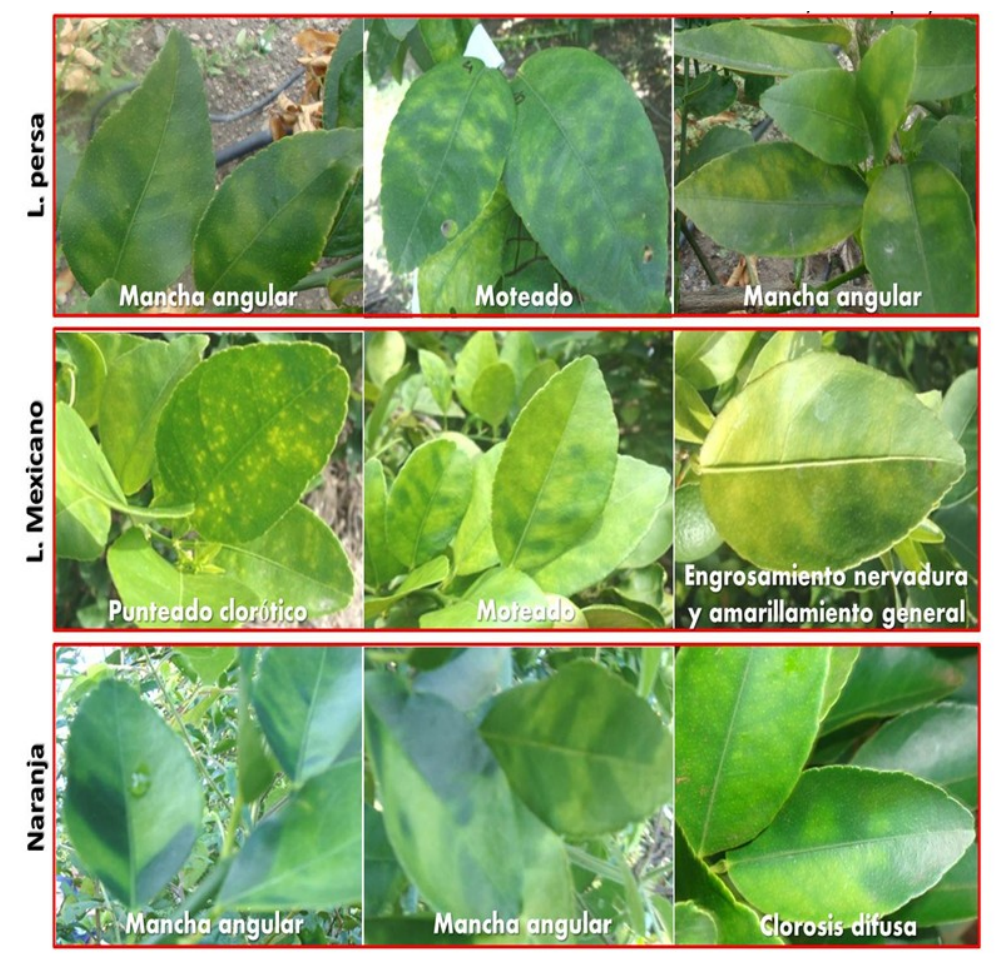
\includegraphics[width=1\textwidth,keepaspectratio=true]{images/C2/1.PNG}
\caption{Síntomas de HLB observados en hojas de limón persa, lima mexicana y naranja dulce, (Fotografía: GIIIC-CP. F. Esquivel y J. Flores, 2010.)}
\end{figure}

\subsection{Modo de transmisión}
%Transmisión y psílidos
Aunque originalmente se pensó que la naturaleza del HLB era viral, posteriormente se tuvo evidencia de que la causa era bacteriana, estas bacterias que se esparcían por los cítricos a través de insectos, estos agentes de transmisión son llamados vectores. Esta infección es diversa y no se limita a algún tipo de clima particular, debido a que a menudo es transmitida por diferentes especies de psílidos que habitan en ambientes diversos. Los cultivos de cítricos que hay en México, tienen las condiciones cálidas y húmedas de las regiones tropicales, de modo que estos cultivos tienen como vector de transmisión al psílido asiático de los cítricos: \textit{Diaphorina citri}, que, como se ha discutido antes, llegó a la región a través de las actividades de la agricultura y es propia de las zonas de siembra.\\

Por otro lado, cuando se observan los cultivos de cítricos en el continente africano, se aprecia que las condiciones son por lo general más frías, y que la bacteria se transmite esta vez por el psílido africano de los cítricos: Trioza erytreae, un insecto intruso al que le favorecen los climas frescos y húmedos y fomentan su crecimiento. Los ejemplares de  Diaphorina Citri nacen de huevecillos que el adulto deposita en los brotes de los árboles, encima y entre los espacios que hay entre las hojas nacientes. Los huevos suelen estar todos concentrados en las mismas ramas de brotes tiernos. Una vez nacen, las ninfas son sedentarias, se establecen sobre estas mismas ramas jóvenes y forman colonias. Para el caso de   Diaphorina citri, se  tiene un periodo embrionario de casi 10 días en un entorno de 15 grados centígrados y de 3.5 días cuando el entorno está a 28 grados centígrados. El tiempo total desde que se deposita el huevo hasta que se convierte en adulto es de aproximadamente 15 días a 28 grados centígrados  y de 49 días a 25 grados centígrados, de modo que las temperaturas entre los 25 y 28 grados centígrados estimulan su desarrollo, sin embargo, un exceso de temperatura tampoco es favorable, pues el psílido no es capaz de desarrollarse en temperaturas que excedan los 33 grados centígrados, teniendo a su vez como cota inferior los diez grados centígrados. A continuación, se muestra una ilustración extraída de la Ficha Técnica del HLB y publicada en 2010 por el SENASICA.

\begin{figure}[H]
\centering
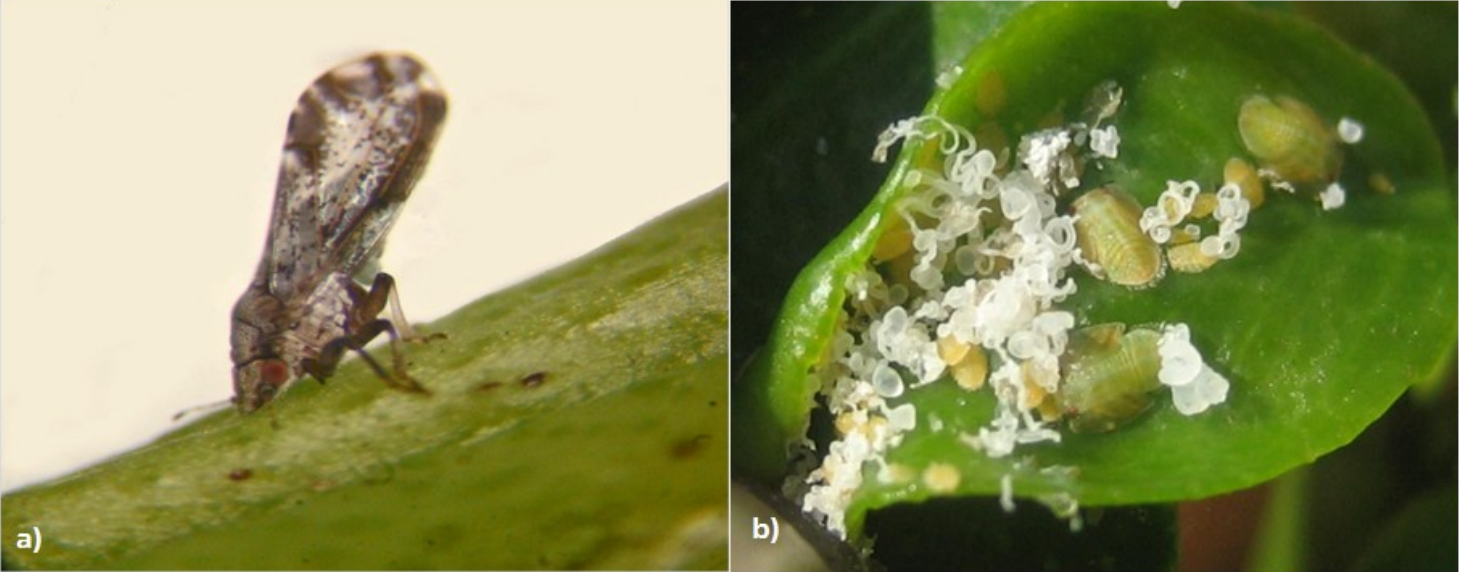
\includegraphics[width=1\textwidth,keepaspectratio=true]{images/C2/2.png}
\caption{a) Adulto, b) Ninfas de Diaphorina citri. Fotografía S. Patiño, R. Lomelí y E. Rodríguez.}
\end{figure}

Los adultos no son capaces de hacer largos viajes mediante el vuelo, de modo que su aparición a grandes distancias es debida más bien a las corrientes de aire, lo que reafirma su naturaleza sedentaria y da un mayor lapso de tiempo para que haya un contagio, tanto de la planta al psílido como del psílido a la planta. El contagio desde la planta al insecto tiene lugar normalmente cuando el psílido se encuentra en un estado ninfal, pero también puede darse cuando éste es adulto, cosa que sucede al momento de que se alimenta de la planta\cite{lopes2006vetor}.


\subsection{Formas de combate al HLB y relevancia económica}
%Control
Más adelante en este trabajo, hay un capítulo entero que aborda la metodología de control usada en México, pero a continuación se mencionan algunos de los métodos y estrategias que son usados en la industria agrícola mundial, siendo algunas de estas estrategias probadas en este trabajo. En primer lugar, se puede hablar del control por plantación de especies inhibidoras, que aunque no es uno de los métodos de control más explorados para el HLB, es de interés porque tiene una notable presencia. Este método consiste en plantar, entre los árboles cítricos, algunos árboles de Guayaba, que tienen propiedades tóxicas para el psílido, de modo que se crean barreras naturales para evitar que el psílido pase a otros árboles. Luego, en contraste con el método anterior, el control químico es de lejos el más utilizado en el campo y el más conocido debido a sus alcances. Otra práctica común es remover los árboles infectados para que éstos no hagan portadores a más psílidos y a su vez contaminen a otros árboles. Una desventaja de esta práctica es que, como se ha visto antes, algunos árboles pueden ser asintomáticos, de modo que es posible tener árboles positivos esparciendo la enfermedad dentro de cierta vecindad sin que se pueda hacer nada; esta estrategia ha sido especialmente relevante en este trabajo, pues tiene un contraste directo con el efecto asintomático.\\
También se ha de decir que existen otras alternativas biológicas de control, por ejemplo, es posible inducir parásitos a las ninfas del psílido, de modo que aumente su mortalidad y su población se vea reducida en virtud de que con esto también disminuyan los contagios de HLB. Finalmente,  es importante decir que los cultivos difícilmente están aislados del todo, esto es, que cuando un campo tiene solo árboles sanos, debería permanecer así por siempre, puesto que ninguno de sus árboles puede contagiar a otro; sin embargo, esto no sucede así en la realidad, de manera que se infiere que la infección por HLB tiene que llegar, necesariamente desde el exterior. Esto no es trivial, debido a que se ha visto que la salud de los cultivos de la región está fuertemente relacionada con la salud de cada cultivo particular\cite{robles2012protocolo}. Esto implica que controlar la infección desde dentro es inútil si el cultivo está en una zona donde hay cultivos con infecciones, puesto que se está mucho más expuesto a las amenazas del exterior, para esto se tienen en México las \textit{Áreas Regionales de Control} (ARCOs) del HLB, de las que se hablará en el siguiente capítulo.

%&Importancia económica
Según los datos en los que se han basado las Normas Oficiales Mexicanas, publicadas por el Gobierno Federal en el Diario Oficial de la Federación, que están encaminadas a combatir el Huanglongbing en México, esta bacteria ya desde 2007 representaba una amenaza para 526 mil hectáreas de cítricos, que implicaban una producción de 6.7 millones de toneladas anuales, con un valor que, ajustado a la inflación según el INEGI, hoy equivaldría a 15 mil millones de pesos, poniendo en riesgo a los 67 mil productores que entonces generaban aproximadamente 70 mil empleos directos y 250 mil indirectos.

%Cierre
Estas han sido algunas características generales del Huanglongbing que son de gran importancia para entender las motivaciones de este trabajo, los objetivos y el objeto de las decisiones tomadas al hacer las simulaciones computacionales. No se profundizará más a partir de aquí en el aspecto interno de este padecimiento, dado que la intención de este trabajo es observar la propagación desde las plantas sanas a las infectadas a través de su vector, de modo que es de poco interés, en este contexto, hablar de cuestiones como el mecanismo mediante el cual la bacteria ocasiona los síntomas de las plantas.


%-----------------------------------------------------------Qué son los sistemas dinámicos 

\section{Los sistemas dinámicos complejos}

Para partir de una base elemental, habrá que acordar qué se entiende por «sistema» y cómo su estudio da pie en ciertas instancias al uso necesario de herramientas computacionales dada su complejidad. En primer lugar, se debe decir que se entiende por \textit{sistema} a cualquier objeto, no necesariamente material, constituido por múltiples componentes que se relacionan entre sí, y evitando profundizar en motivos filosóficos, se puede entender de forma intuitiva a un sistema como \textit{un conjunto de elementos que no puede ser estudiado a través del estudio individual de estos elementos}. Esto implica que son precisamente las relaciones entre los elementos del sistema lo que le da las características emergentes que lo convierten en algo más que la simple suma de los elementos que lo conforman. Si se piensa, por ejemplo, en volúmenes de pintura rosa; la mezcla de estos volúmenes de pintura rosa será otro volumen pintura rosa y nada más. Salvo el hecho de que el volumen resultante será más grande que el anterior, no existen fenómenos que lo hagan sustancialmente distinto de los volúmenes que lo conforman. Básicamente: la mezcla de pintura rosa es más pintura rosa, vaya descubrimiento. Sin embargo, esto no es trivial, porque esto no ocurre, por ejemplo, si se presta atención a las partículas de algún material, cuya mezcla formaría algún gas o, líquido o, cualquier otro tipo de material con propiedades distintas a las de la partícula que la conforman, este hecho es nada menos que el inicio de la \textit{física molecular}, pues como se ha visto ya, entender las leyes que rigen el comportamiento de las partículas, por ejemplo, su \textit{momento}, no es suficiente para entender el fenómeno macroscópico. Finalmente se ha de decir que es interesante pensar en que un objeto que no sea un sistema, uno que en efecto sí se constituya a sí mismo, sería necesariamente un objeto \textit{autorreferencial}, aunque como se ha dicho, no es competencia de este trabajo entrar en honduras filosóficas, así que más allá de este hecho curioso y dada esta poco rigurosa definición, podemos estar firmes en la idea de que los sistemas y sus propiedades no pueden ser estudiados a través del estudio individual de sus partes, y teniendo esto en mente, podemos continuar con el estudio de los sistemas dinámicos. Los sistemas dinámicos son simplemente aquellos sistemas que cambian de estado a través del tiempo sin detenerse, de modo que pueden ser descritos en función de él. Muchos de los fenómenos cotidianos son sistemas dinámicos; como el movimiento de los cuerpos en física, el crecimiento de alguna población en biología o la evolución del PIB de alguna región en economía. También es cierto que otros ámbitos del conocimiento no se pueden abordar desde un punto que involucre al tiempo, como las leyes de un estado en derecho, la lógica formal en filosofía y hasta el equilibrio con el que cuelga un candelabro de algún teatro, siendo este último ejemplo un caso de especial interés dado que de él puede decirse que su movimiento tiende a cero conforme pasa el tiempo. Es posible sacar a este candelabro de su equilibro y hacerlo balancearse, incluso se puede estudiar su movimiento, pero finalmente siempre volverá a colgar en reposo. Decimos que este sistema tiende a un \textit{estado estacionario}, esto es, que sus variables no cambian con el tiempo.\\
Por otro lado, dentro de los sistemas dinámicos existe una parte que son los sistemas complejos, los sistemas complejos se caracterizan porque las relaciones que hay entre sus elementos añaden información extra, esto es que, a diferencia de un sistema común, no sólo no podemos entenderlos a través del estudio individual de sus elementos, sino que tampoco podemos estudiar individualmente las relaciones entre ellos, haciendo que carezca de sentido cualquier tipo de enfoque particular cuando se pretende entender un sistema como estos, de modo que las técnicas para estudiarlos tienen que ser algo más sofisticadas. Definamos vagamente a un sistema complejo como fuera definido por Herbert Simon en 1962 \cite{weaver1991science}: una red formada de elementos cuya interacción suele ser  \textit{no lineal}. Los sistemas complejos tienen la capacidad de manifestarse y cambiar mediante la \textit{autoorganización}, de una forma tal que no son absolutamente homogéneos pero tampoco son absolutamente aleatorios, y es esto lo que induce esas características emergente a nivel macroscópico de las que hemos hablado antes. Finalmente, aunque no entraremos en este terreno, es de interés decir que hay un tipo más sofisticado de sistema complejo; el sistema caótico. Un sistema caótico es un sistema dinámico complejo en el que pequeños cambios en sus variables iniciales, producen eventualmente grandes cambios en las variables finales. Esto hace que el estudio de estos sistemas no pueda ser abordado de la forma en la que se han estudiado otros en el pasado dado que cualquier sutil error de medición puede cambiar drásticamente la predicción de su comportamiento. El ejemplo típico es el del clima, se ha visto que al intentar hacer predicciones del comportamiento del tiempo en los próximos días, estas coinciden para los primeros días, pero conforme tratamos de predecir más y más días en el futuro las predicciones difieren arbitrariamente una de otra. Podríamos decir que con los modelos actuales del clima, no se puede hacer una predicción razonable sobre cómo estará el tiempo dentro de más de tres días, y esto se debe justamente a que el sistema es caótico y que pequeños cambios en las mediciones que hagamos para su predicción hacen que los resultados difieran tanto, que simplemente sería más acertado usar la estadística meteorológica.\\
Volviendo al tema que ocupa a esta sección, se ha de mencionar que las cualidades de las que gozan los sistemas mencionados anteriormente son cualidades presentes en muchos sistemas del mundo real, como los procesos fisiológicos involucrados en los organismos, las redes sociales, los fenómenos macroeconómicos, las cadenas alimenticias, los procesos neurológicos, los mercados de valores, el desarrollo del poder político y las civilizaciones, y un afortunadamente largo etcétera. Hay que puntualizar que no se debe confundir «complejo» con «complicado», existen sistemas que carecen de complicación, es decir que son simples, pero su comportamiento es complejo, y por otro lado también existen sistemas cuyo comportamiento no es complejo a pesar de ser tremendamente complicados. Además, algunos sistemas pueden ser estudiados individualmente; sistemas como dados cayendo o gases, pueden ser estudiados por la teoría de la probabilidad y física molecular respectivamente sin tener complejidad a pesar de que el fenómeno sea bastante complicado, y esto es porque se estudian sus componentes como independientes. En el otro lado, están por ejemplo los cuerpos rígidos o el lanzamiento simultáneo y combinado de dados, que tampoco son sistemas complejos, y pueden ser estudiados como sistemas acoplados. Sin embargo existe una zona en la que no hay sistemas completamente independientes o completamente acoplados, estos sistemas están en una zona que parece tener algo de organización dentro de su naturaleza compleja, esta naturaleza interdependiente puede ser abordada desde las matemáticas y la computación . Históricamente hay dos conceptos fundamentales que están involucrados en los sistemas complejos; los fenómenos emergentes y la autoorganización. En primer lugar, el concepto de los fenómenos emergentes llegó más bien de una forma filosófica, como resultado de los diversos procesos naturales en los que las propiedades del sistema a nivel macroscópico no pueden derivarse de leyes o modelos a nivel microscópico. Por ejemplo, para la medicina es trivial tener la certeza de si una persona está consciente o no, pero difícilmente podrá explicar de una forma precisa a nivel químico y físico cada uno de los procesos involucrados en la consciencia, similarmente esto sucede con las sociedades, es fácil decir qué regiones tienen un mayor índice de Desarrollo Humano o la mayor tasa de mortalidad infantil, pero difícilmente se podrá explicar exactamente qué incidentes particulares provocan estos hechos. A pesar de que en la elaboración de este texto se han encontrado varias definiciones distintas del concepto de “fenómenos emergentes”, por lo que parece no haber un consenso claro, hay algunas ideas comunes en la mayoría de estas definiciones consultadas, en primer lugar, el hecho de que los fenómenos emergentes (a veces también llamados emergencia o surgimiento) existen propiedades a escala macroscópica que son sustancialmente distintas de lo que se derivaría en principio de las leyes con las que se describe la escala macroscópica, de modo que hay emergencia de propiedades que no estaban evidentemente ahí cuando el análisis era puramente microscópico. Justamente, en este punto yace lo que le da interés a los fenómenos emergentes, que no son triviales, que hasta hoy no se conoce alguna forma simple de descubrir cómo se relacionan las propiedades de los elementos individuales del sistema que conforman. La autoorganización es también otro punto de importancia fundamental en el estudio de los sistemas complejos, que aunque pudiera parecer, no es lo mismo que las propiedades emergentes. La diferencia es que las propiedades emergentes son un asunto relacionado solamente con la escala (en tamaño), mientras que la autoorganización está relacionada además con el tiempo. De modo que se dice que algo es autoorganizado cuando al cabo de un tiempo  aparece espontáneamente un orden en el sistema en forma de alguna estructura o comportamiento regular a nivel macroscópico, y aunque parece que esto implicaría que la autoorganización es una paradoja o que contraviene la segunda ley de la termodinámica, esto no es así, desde luego, como lo veremos a continuación. A estas alturas el lector habrá pensado ya en varios sistemas cotidianos, naturales o sociales que exhiben un comportamiento de autoorganización, sin embargo habrá de estar tranquilo porque hasta ahora parece claro que ninguno de esos sistemas viola realmente la inexorable segunda ley de la termodinámica, y el secreto está en que estos son sistemas que no están ni cerrados ni aislados, tal como lo exigiría esta ley.
Para sintetizar lo anterior, los sistemas complejos son aquellos en los que surgen estructuras y comportamientos no triviales en sus propiedades macroscópicas como consecuencia de sus propiedades microscópicas, ya sea después de algún tiempo o al instante.
%Cerrar hablando de determinismo
Para terminar con esta sección, es bueno mencionar que la forma en la que se han estudiado tradicionalmente los sistemas físicos es \textit{determinista}, esto es que se tiene como un axioma la idea de que

%-----------------------------------------------------------Qué es la Simulación Computacional y el modelado

\section{La simulación computacional y el modelado matemático}
%Modelado matemático
«\textit{Ceci n'est pas une pipe}» (Esto no es una pipa), dice con grandes letras aquel cuadro surrealista de René Magritte en el que flagrantemente dibuja una pipa. Y en efecto, aquella obra del pintor francés no es una pipa sino una representación de una pipa, además de un doloroso recordatorio de que \textit{símbolo} y \textit{referente} son términos que no se deben confundir. Anteriormente no entramos en honduras filosóficas ni tampoco entraremos aquí en honduras lingüísticas, así que podemos ser simples y decir que los símbolos son los signos que usamos para evocar objetos o referentes, pero no son el objeto en sí, del mismo modo que un dibujo de una papa no es una papa. Y sí, esto es relevante para lo que sigue porque en ciencia sucede algo muy similar: toda la literatura que existe sobre los fenómenos naturales no es el fenómeno natural en sí, y más desolador aún, las imágenes mentales que se hacen los científicos de esos fenómenos tampoco son el fenómeno en sí. Es entonces osado decir que la labor del científico es la de entender la realidad, más bien esta labor se limita solamente a construir modelos cuyas predicciones sean consistentes con las observaciones experimentales en el mejor de los casos. Sin embargo, esta es seguramente la más noble de las labores humanas; la observación de la naturaleza, el modelado de sus fenómenos y la rigurosa prueba de estos modelos de forma experimental. La ciencia es modelar, y modelar es, de una forma poco rigurosa; crear una representación simple de un sistema.\newline
En cierto modo los seres humanos, para interactuar con el exterior y constituirse como tal, deben crear modelos en su mente, las tareas cognitivas cotidianas están basadas en modelos del exterior. Los modelos de la ciencia, sin embargo son más sofisticados, no son algo que surja espontáneamente en la mente, son un esfuerzo colectivo que trasciende las vidas de los científicos y son el único contacto racional que se tiene con la inclemente realidad, además de que en última instancia, todo este conjunto modelos, esta ciencia, sirven para controlar la naturaleza. Los modelos son a menudo una descripción centrada en el comportamiento de los sistemas, se enfocan en las características en puntos fijos del tiempo, ejemplos de esto son los mapas o diagramas, aunque también existe un enfoque que aborda el estudio de los sistemas desde el punto de sus reglas más que de su descripción, como las leyes de Newton, por ejemplo. Este es un enfoque dinámico que más que describir, explica el comportamiento de los sistemas, este tipo de abordaje de los problemas permite hacer predicciones sobre ellos, aunque ambas son igual de relevantes en la ciencia. Naturalmente, este trabajo tiene un enfoque que pretende explicar y predecir.\\
Claramente la labor de modelar la realidad no es sencilla, pero cuando se trata de modelar sistemas complejos, esto se suele complicar más, y esto se debe a lo hablado anteriormente, son las características propias del sistema como las propiedades emergentes, la autoorganización o los comportamientos no lineales, las que complican el modelado de estos sistemas. Para los físicos, es una herramienta confiable hacer simplificaciones y suposiciones al modelar, y esto suele ser una herramienta muy poderosa para la mayoría de sistemas típicos, por eso es común que la forma de abordar esto considere solamente cierta escala, y que si el razonamiento está dentro de una estala, se desarrolle ahí pero que nunca escale a otra, de modo que las secuencias en el proceso de pensar siguen el curso de la causalidad de una forma lineal. Y esto es algo que se ha de evitar cuando se pretenda comprender sistemas complejos, en esta instancia se debe considerar que existen muchos elementos interactuando entre sí pero independientemente, hecho que genera las ya discutidas repercusiones en otras escalas. Dicho esto, finalmente podemos deducir que los sistemas complejos son por lo común poco intuitivos y difíciles de entender, siendo esto incluso imposible a veces.\\
Pero claramente esto no puede terminar así, la conclusión no puede ser que estudiar estos sistemas es difícil y ya. Es cierto que las habilidades y la experiencia para encontrar las relaciones entre lo macroscópico y lo microscópico no son comunes a todos, pero sí es cierto que se pueden adquirir y desarrollar, y esto es tan simple como la práctica. Evidentemente es complicado acceder a las propiedades microscópicas y macroscópicas de muchos sistemas para adquirir práctica, sin embargo, las herramientas computacionales hacen que esto sea accesible y escalable. Se puede siempre construir un modelo propio al gusto con cada detalle, con cada regla y propiedad microscópica escritas en el código de la simulación para después ejecutarla y observar su comportamiento en un nivel macroscópico, que tendría que manifestar esos deseados fenómenos emergentes y de autoorganización.\\
En este trabajo seguimos ciertos criterios que han dirigido el desarrollo de la simulación, en primer lugar y como pieza clave de la ciencia, se ha buscado que el modelo pueda predecir en cierta medida razonable la realidad, sin esta característica este modelo sería de ningún interés científico además de que en la práctica tampoco tendría utilidad, si las predicciones del modelo no coincidieran o se acercaran consistentemente a los que se observa a través de la experiencia, entonces significaría que no es una representación de la realidad, que es como hemos visto antes, su único fin, de modo que su única utilidad es la de saber en qué dirección no seguir. Dado esto, se nota fácilmente la importancia de poner a prueba los modelos desarrollados y demostrar su validez; esto tanto en el ámbito de las suposiciones de las que se ha partido en su desarrollo como de las predicciones que obtenemos de él, y esto se logra a través de verificar que toda suposición sea consistente con el resto del conocimiento científico. Como probablemente el lector haya experimentado ya, es común encontrarnos con modelos de la realidad poco científicos, que a pesar de que algunos pueden rebuscados y en buena medida, libres de contradicciones, parten de bases falsas o de las que no se puede verificar la veracidad, de modo que todo el sistema carece de sentido científico, como sucede con las llamadas seudociencias.  Esto se agrava con los sistemas en los que es difícil o directamente imposible realizar alguna comparación entre la predicción que da el modelo y la evidencia de forma cuantitativa. De modo que un modelo que tenga estas características es difícil de poner a prueba y puede ser susceptible de no ser riguroso, sin embargo se ha de procurar prestar atención a los principios de los que se parte. Es en este punto donde se ha de hablar de la segunda pieza clave en este desarrollo,  buscar la simplicidad tanto como la validez. Es sensato notar que en la medida en la que se aumenta la complejidad del modelo, se suele obtener un mejor acercamiento a los datos que se observan experimentalmente, sin embargo esto puede ir en detrimento de la simplicidad, y esto hace que el modelo pierda, generalización para cuando se trata de predecir otros casos. De modo que se necesita un equilibrio para poder describir en la medida de lo posible lo general tanto como lo particular.\\
En efecto, buscar la simplicidad es algo fundamental en la construcción de un modelo, una razón es la de obtener descripciones cortas puesto que facilitan el trabajo y requieren menos recursos, pero también hay una razón más profunda, que la explicación más sencilla de las cosas se suele tomar por la más probable, y aunque no haya alguna prueba de que esto sea cierto en lo particular, suele funcionar en la mayoría de los casos. Es una práctica común inclinarse por las explicaciones más cortas siguiendo al famoso principio de la navaja de Ockham; en igualdad de condiciones, la explicación más simple suele ser la más probable. Además los modelos más simples son más fáciles de recordar y de aplicar, de modo que siempre que sea posible prescindir de algún parámetro o suposición debería hacerse, tal como se ha hecho en este modelado del HLB.
%La Simulación Computacional

La simulación que es objeto de esta tesis ha sido escrita en el lenguaje de programación Python, y se usarán las siguientes líneas  para describir sus ventajas y su importancia en el área de la simulación computacional y el modelado matemático, se hablará también de algunos grandes proyectos escritos en este lenguaje, pasando por la historia, no sólo de Python sino de la simulación computacional en general, para finalmente aterrizar en el modelado y análisis de sistemas complejos y particularmente del modelado basado en agentes individuales, que es el tipo de modelado que se usa en este trabajo. Por último, como finalidad de todo esto, haremos la obligada descripción del código de esta simulación.
Comencemos hablando de Python, un lenguaje que apareció por primera vez en febrero de 1991, hace treinta y un años, y que desde entonces ha ido cobrando relevancia hasta el gran ascenso de popularidad que ha tenido en los últimos años y que lo ha llevado a ser hoy día uno de los lenguajes de programación más populares entre la comunidad de desarrolladores de software. Python es un lenguaje orientado a objetos, de alto nivel, de \textit{tipado} fuerte y dinámico, estas características lo hacen perfecto para lo que atañe a nuestros intereses y por eso las describiremos una a una.
Es importante mencionar que Python es un lenguaje que admite múltiples paradigmas de programación, pero nosotros nos centraremos en el paradigma de la programación orientada a objetos. Que sea orientado a objetos es, sin mucho tecnicismo, que en este lenguaje podemos crear dentro del código unas entidades llamadas \textit{objetos}, que pueden ser pensados como los objetos de nuestra vida cotidiana, por ejemplo un árbol. Estos objetos, igual que los de la realidad, tienen características propias, a las que llamamos \textit{atributos}; por ejemplo su tamaño o el número de hojas para el caso del árbol, y también pueden tener \textit{funciones}, que pueden ser vistas como acciones de las que nuestro objeto forme parte y que a diferencia de los atributos que sólo son un registro de alguna característica de nuestro objeto, las funciones implican un proceso computacional, por ejemplo, el crecer o el perder todas las hojas para el caso del árbol pueden ser funciones del objeto. Esto hace que nuestro código se parezca más a la realidad y logra que programar en Python sea bastante intuitivo y que la simulación y el modelado se faciliten. Para aportar un poco más de información sobre cómo funciona intuitivamente la programación orientada a objetos, veamos un caso que ha surgido en esta simulación, en la que tenemos el ejemplo del objeto «Árbol», y del objeto «Psílido», que tiene algunos atributos como su posición que corresponde a la posición del árbol que la aloja, y si está infectada o no; además tiene la función de volar a otras posiciones y de infectar al árbol que la aloja. Estas dos últimas funciones modifican dos atributos, la primera modifica el atributo posición de el propio psílido, y el segundo modifica el atributo que nos dice si el árbol está o no infectado, desde luego que para que nuestra simulación sea de interés, el procedimiento para modificar estas variables no puede ser arbitrario y tiene que procurar comportarse como lo haría la propia naturaleza, de modo que de aquí se puede inferir que dentro de nuestras funciones de los objetos tiene que haber una buen modelado matemático basada en un conocimiento realista del fenómeno que se está describiendo, así que usando un lenguaje orientado a objetos, la labor se reduce a crear los objetos y luego plasmar en ellos las propiedades y comportamientos que se presuman como reales. Que sea de alto nivel puede ser entendido de una forma intuitiva como que su sintaxis es más abstracta, que se asemeja más al lenguaje que tenemos las personas que al lenguaje de las máquinas, encima Python tiene una gramática sencilla, puesto que prescinde de muchos símbolos engorrosos como el punto y coma al final de cada sentencia que se usa en ortos lenguajes de programación. El tipado fuerte se refiere a que el lenguaje distingue de una forma rigurosa los tipos de variables, por ejemplo, un número entero como la cantidad de psílidos de  que aloja un árbol, de un valor booleano (Verdadero o Falso) como lo puede ser si el árbol está infectado o no. A pesar de esta marcada distinción, Python tiene también un tipado dinámico, esto quiere decir que a diferencia de otros lenguajes de programación, en este no es necesario declarar al inicio del programa qué variables y de qué tipo de se usarán, haciendo que crear una variable sea más sencillo.
Por lo escrito anteriormente es claro ya que Python es una gran tecnología que goza además de una gran popularidad, pero este lenguaje es especialmente usado en la simulación de sistemas dinámicos complejos, y un ejemplo ilustre por su valor se puede encontrar en el \textit{PyCX} \cite{sayama_2013} que es un repositorio alojado en GitHub que contiene múltiples códigos de muestra sobre simulación de sistemas complejos, con un enfoque educativo y para la investigación. Este repositorio tiene como finalidad ser el punto de partida de proyectos para los estudiantes e investigadores que comiencen a incursionar en el campo del desarrollo de software para estudiar sistemas complejos, incluyendo códigos muestra de mapas iterativos, ecuaciones diferenciales tanto ordinarias como parciales, autómatas celulares, análisis de redes, redes dinámicas y modelos basados en agentes individuales también llamados «ABM», siendo estos últimos de especial interés para este trabajo.
\chapter{Métodos de Control del Huanglongbing en México}

En este capítulo, se describen las normas y los mecanismos institucionales para el tratamiento del HLB en México, así como el protocolo que se instruye seguir a los agricultores ante la detección de un árbol con evidentes síntomas de la enfermedad, además, se muestran los métodos empleados cuando existe sospecha de un brote. Este capítulo da fundamento a la forma en la que se han simulado el campo y los métodos de control aplicados en él en este trabajo, puesto que, como se verá más adelante en el siguiente capítulo, el objetivo principal de este experimento es poner a prueba las medidas en el combate y prevención de las infecciones por esta enfermedad en México. El Capítulo analiza los manuales y protocolos publicados por la autoridad correspondiente, con la idea de tener información oficial de la forma en la que se trata a esta enfermedad en el país, y de este modo tener una simulación congruente.\\
En México, en el año en el que se escribe esta tesis, es atribución de la Secretaría de Agricultura y Desarrollo Rural (SADER), llamada en sexenios pasados Secretaría de Agricultura, Ganadería, Desarrollo Rural, Pesca y Alimentación (SAGARPA), el establecimiento de las medidas fitosanitarias pertinentes en virtud de la  prevención y el control de las plagas capaces de potencialmente mermar las cosechas de vegetales, así como sus productos y subproductos. Es importante puntualizar que los productos \textit{fitosanitarios} son, en general, aquellas sustancias capaces de prevenir o combatir a las plagas, que para el caso que ocupa a este trabajo, suelen ser los insecticidas usados para combatir al vector transmisor \textit{Diaphorina citri}, o en un caso más remoto; bactericidas o antibióticos para atacar directamente a la bacteria que causa la enfermedad. Además, existe un organismo descentralizado de la SADER, el SENASICA, cuyo fin es el de proteger los recursos agrícolas de plagas y enfermedades de cuarentena. Además, se encarga de la regulación y el fomento de los sistemas de reducción de riesgos de contaminación de alimentos, para dar certeza a los productos vegetales y animales, así como sus derivados, para el comercio nacional e internacional.\cite{cortez2010control}

\section{La Campaña contra el Huanglongbing de los Cítricos}

Dado que el SENASICA es el responsable de implementar las acciones encaminadas a la prevención, control y erradicación de las plagas en el territorio nacional, particularmente para el caso del Huanglongbing, se han tomado algunas medidas fitosanitarias como: vigilancia epidemiológica en huertos comerciales y zonas urbanas, así como el control químico y biológico del vector, tanto en jardines como en huertos comerciales de zonas en las que existe concurrencia de focos de infección. Este conjunto de acciones constituyen a la Campaña contra el Huanglongbing de los Cítricos. Las zonas a las que se dirige esta campaña, son denominadas \textit{ARCOs}. El sentido de los ARCOs es el de agrupar todas las actividades de vigilancia, control biológico y control químico en un área estratégicamente definida en extensión y forma, en virtud de reducir la posibilidad de que los focos de la epidemia alcancen mayores proporciones, y es en este contexto que es de interés revisar la metodología usada por esta campaña para la detección del Huanglongbing, así como las acciones a realizar ante la detección de esta enfermedad, tanto en las plantas como en los psílidos infectivos que habiten en huertas comerciales y zonas urbanas. Finalmente, esta sección busca puntualizar los criterios para la búsqueda y control de los árboles infecciosos.

\subsection{Búsqueda y detección del Huanglongbing}
A lo largo del país, a través de los huertos comerciales y domésticos, tanto en las plantas de cítricos como en algunas ornamentales, existen dos formas de detectar el HLB. La primera es indirecta, mediante la colecta de los insectos transmisores que son posteriormente analizados para detectar a la bacteria causante. En la forma directa, se da la búsqueda de síntomas de primera mano en la materia vegetal.\\ El proceso en los huertos comerciales de las zonas citrícolas que no tienen presencia de la enfermedad, es homogéneo, sin embargo, el muestreo en los huertos es priorizado dependiendo de algunas condiciones que los hagan más propensos a contraer la enfermedad. Los criterios son varios, como que en los huertos existan plantas que tengan menos de 10 años de edad, que se localicen junto a lagunas u otros cuerpos de agua, o que la huerta sea joven y esté próxima a una adulta; otras condiciones para priorizar una huerta son: que se localice cerca de una frontera, costa, área urbana o algún centro donde se concentren cítricos, que colinde con estados o zonas con presencia de HLB o incluso las carreteras que conducen a ellos.\\
El primer paso para la detección indirecta es la toma de una muestra, en cada huerto, de cierta cantidad de psílidos adultos. La muestra se hace manualmente, por lo general con una aspiradora o algún otro instrumento que asegure a los insectos, que posteriormente son colocados en viales con alcohol etílico y son etiquetados. Una vez colectadas las muestras, éstas son enviadas al laboratorio con la menor demora posible, para de estar en condiciones de detectar oportunamente cualquier caso positivo y con ello encontrar los posibles focos de infección. El personal que toma las muestras se auxilia de un teléfono en el que registra la geolocalización de dichas muestras.\\
La minoría de los huertos en los que se colectan las muestras son mayores a cinco hectáreas, habiendo incluso entidades en las que, debido a que los huertos son pequeños, las muestras son en su totalidad en huertos menores a cinco hectáreas. Si el huerto es menor a cinco hectáreas, el muestreo es metódico, y se colectan entre 5 y 10 insectos de cada planta. En total se eligen veinticuatro plantas de la siguiente forma: supongamos que el huerto tiene forma de cuadrilátero y se elige una cara de éste, preferentemente la que recibe predominantemente el soplar del viento la mayor parte del tiempo, en el borde de esta cara se elige el árbol que esté en alguna de las dos esquinas, luego se dejan tres árboles a lo largo de este borde y se vuelve a muestrear, de modo como se ve en la figura 3.1. Una vez trazado el primer patrón, se toman los dos árboles que estén en la parte media de la línea de muestreo, y desde ellos se sigue con el mismo procedimiento, pero esta vez con dirección al centro del huerto, lo que resulta en un patrón en toda la arista del cuadrado en el que hay un muestreo cada tres árboles, a esto se le llama método en «T».

\begin{figure}[H]
\centering
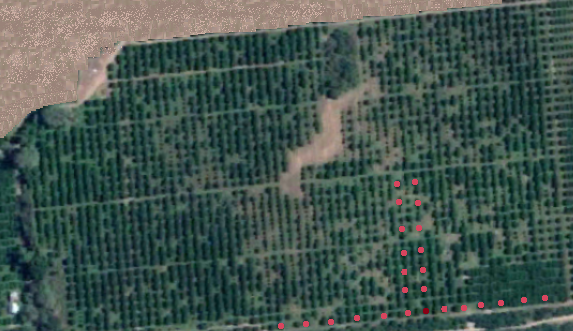
\includegraphics[width=0.6\textwidth,keepaspectratio=true]{images/C3/T.png}
\caption{Ilustración del método en «T». Una huerta cuyos árboles examinados se marcan en rojo.}
\end{figure}

Cuando los huertos son mayores a cinco hectáreas el método es muy parecido, salvo por el hecho de que en este caso se emplea dos veces el procedimiento descrito anteriormente, aplicando el segundo en la cara opuesta a la cara en la que se aplicó el anterior, esto se puede observar en la figura 3.2.

\begin{figure}[H]
\centering
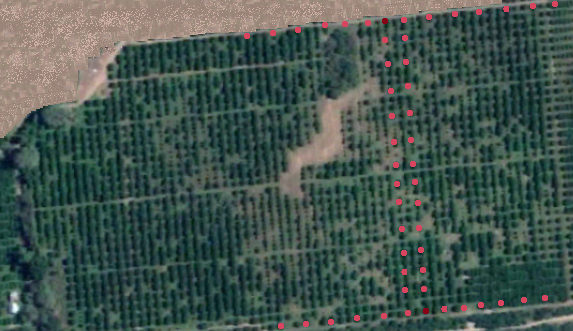
\includegraphics[width=0.6\textwidth,keepaspectratio=true]{images/C3/T2.png}
\caption{Ilustración del método en doble «T».}
\end{figure}

En las zonas urbanas existen rutas de muestreo que se recorren mensualmente, las zonas que recorren estas rutas están constituidas por una media de tres poblaciones o comunidades en las que no existe presencia de la enfermedad pero sí del psílido, se pone especial interés en los árboles de limón mexicano y se toma una muestra por cada comunidad, pudiendo contener hasta cien individuos, y tomando muestras de cinco árboles distintos en los períodos de alta infestación. Los lugares de recolección son camellones, jardineras o parques. 

\subsection{Protocolo ante la detección de muestras positivas a Candidatus Liberibacter}
Ante la detección de casos positivos en las muestras tomadas durante los procedimientos descritos anteriormente, ya sea a través de las muestras de psílidos adultos o en las del material vegetal con síntomas (que se detallan e ilustran en el capítulo anterior: Conceptos Preliminares), existen diferentes medidas a tomar, dependiendo del caso de la detección, pero más allá de qué medidas se implementen, se debe tener presente que es la Dirección General de Sanidad Vegetal la autoridad encargada de gestionar las acciones procedentes.\\

%4.1
Cuando se detectan psílidos infectivos en huertos comerciales, después de algunos procedimientos institucionales en los que no se profundizará, se designa a un responsable, miembro de algún organismo gubernamental, para que coordine las acciones a llevar a cabo para hacer frente a la amenaza. Estas actividades incluyen colectar psílidos o directamente comenzar con su control, y de ser necesario, la búsqueda de síntomas en el área de influencia de la detección, y posterior a esto se rinde un informe en un plazo no mayor a diez días hábiles a partir de la conclusión de estas actividades.\\
La exploración para la detección de síntomas en los cítricos comienza con la revisión de la totalidad de los árboles que conforman el huerto en el que se ha detectado el brote; es importante enfatizar que esta revisión se limita a buscar síntomas, algo que contribuye a combatir el brote pero no da una certeza total, dado que, como se ha dicho antes, algunos árboles muestran sus síntomas mucho tiempo después de ser portadores. Si se encuentran síntomas en un árbol, se colectan algunas piezas de material vegetal y se analizan, y en caso de que se confirme un resultado positivo, se instruye al productor realizar una aplicación de insecticida contra el vector. Además, se \textit{delimita el brote} y se promueven las \textit{actividades para su manejo}, dos temas que se tratarán más adelante. Si los resultados obtenidos después de estas acciones no son los deseables, la huerta es considerada como un «punto rojo» para muestreo y diagnóstico, por lo que se instruye nuevamente al productor aplicar insecticida contra el vector.\\
El muestreo de psílidos se hace mediante la colecta de ellos de forma simultánea a la búsqueda de síntomas, descrita anteriormente. La forma de recabar a estos ejemplares es parecida a la descrita anteriormente, se toman veinte plantas, esta vez dejando dos árboles entre cada árbol elegido, en lugar de tres como en el caso anterior, pero manteniendo la misma estructura perpendicular y colectando también de cinco a diez insectos por árbol. Si hay alguna localidad urbana a menos de un kilómetro de la huerta donde se detectó la muestra positiva, existe una alta probabilidad de encontrar HLB en ella, de modo que esta también debe ser analizada. Si alguna huerta reincide en tener psílidos infectivos, la autoridad competente notifica al productor la responsabilidad del control del psílido.\\
\begin{figure}[H]
\centering
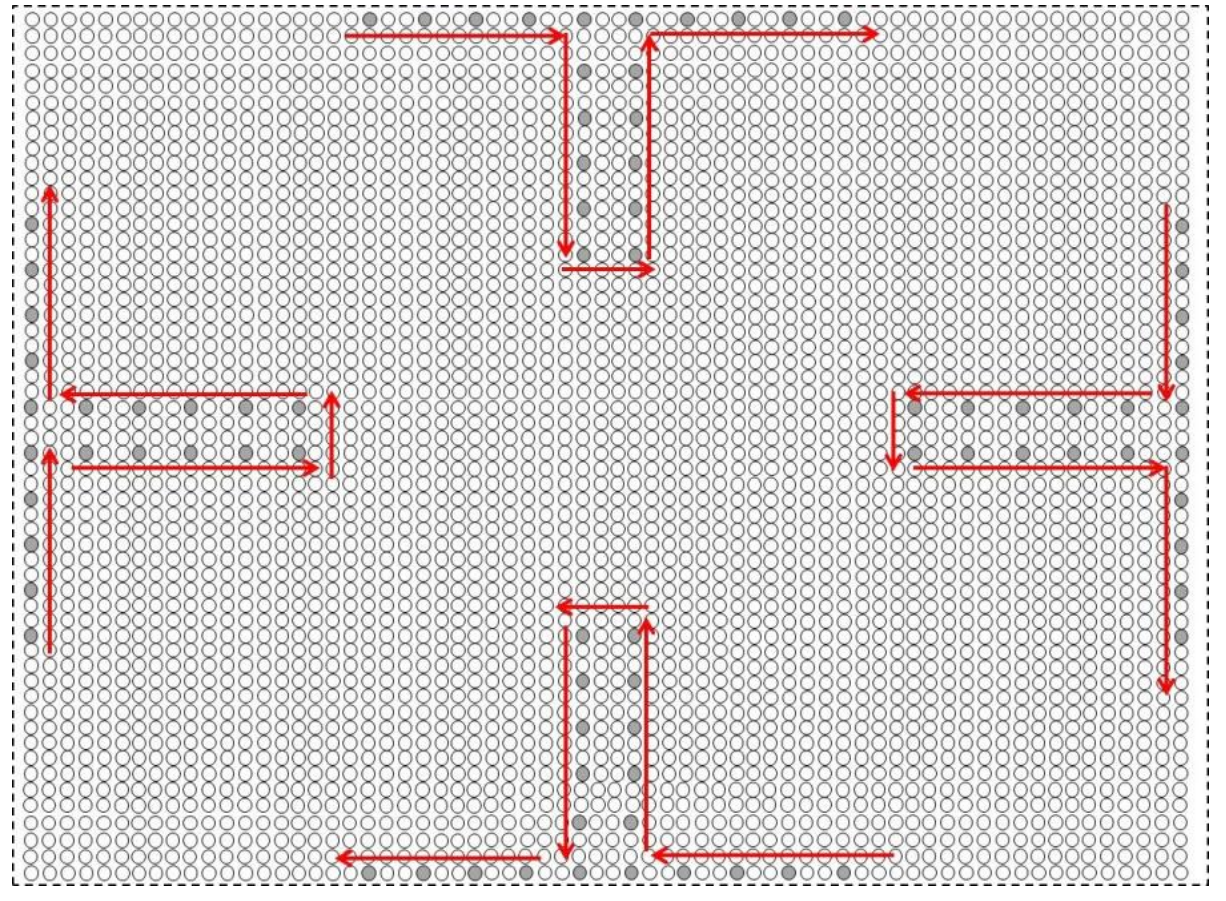
\includegraphics[width=0.8\textwidth,keepaspectratio=true]{images/Norm/MT.png}
\caption{Ilustración del método en T. Manual operativo de la Campaña contra el Huanglongbing de los Cítrico}
\end{figure}
%4.2
Cuando se detectan psílidos infectivos en rutas de muestreo de zonas urbanas, se revisa la totalidad de las plantas de la localidad donde se detectó la infección y se toman muestras de materia vegetal de las plantas que presenten la sintomatología característica del HLB y paralelamente se capturan algunos psílidos por cada manzana de casas. Si las pruebas resultan positivas, la autoridad aplica insecticida en toda la manzana y en las colindantes. Si los resultados son negativos, solamente se aplica insecticida puntualmente en las plantas con psílidos positivos.\\
%4.3
Respecto a la delimitación de los brotes de HLB, existen tres ámbitos, en primer lugar, naturalmente se empieza con la formación de brigadas para su posterior movilización, y entonces se implementan las acciones para delimitar el foco inicial en los sitios con detecciones, esto a un nivel local, y para un nivel regional se emprenden las acciones encaminadas a delimitar los focos en toda la comarca. La formación y movilización de las brigadas comienza con la notificación oficial  de la confirmación de HLB, y la autoridad competente pone en marcha a los equipos con los insumos necesarios que llevarán a cabo las acciones, estas brigadas contarán con técnicos para reconocer los síntomas de HLB y los instrumentos necesarios para el registro de la localización de las plantas sospechosas\\
En el segundo ámbito, en el encaminado a delimitar el foco inicial de los sitios con detecciones, se realiza una exploración intensiva en el huerto donde se detectó el cítrico positivo, siguiendo la figura 3.4:\\

\begin{figure}[H]
\centering
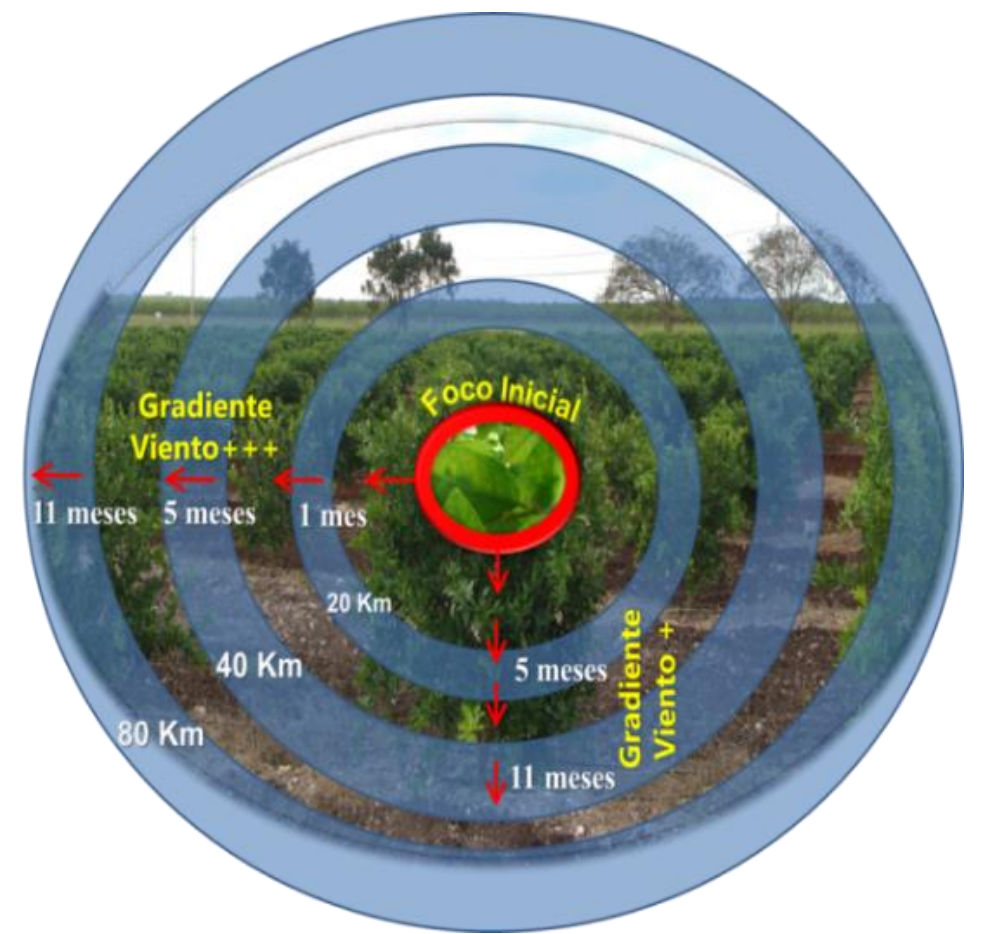
\includegraphics[width=0.5\textwidth,keepaspectratio=true]{images/Norm/figura 7-10.png}
\caption{Delimitación del foco inicial. Manual operativo de la Campaña contra el Huanglongbing de los Cítrico}
\end{figure}

En un siguiente nivel en escala, las acciones para determinar los focos regionales están condicionadas por las direcciones de los vientos dominantes, que favorecen la dispersión del HLB a nivel regional. La delimitación de estos focos de infección se hace mediante recorridos en rutas de muestro que se trazan a partir de la detección de una planta positiva en muestreos cada veinte kilómetros.

%4.4, 4.5
Finalmente, la divulgación y el manejo del brote son de suma importancia y son responsabilidad de la autoridad, esta divulgación debe hacerse oportunamente entre los productores, organizaciones relacionadas con la producción y las organizaciones nacionales de otros países a través de la Organización Norteamericana de Protección a las Plantas (NAPPO). Para manejar los brotes de HLB, en principio, habría de bastar con la localización y eliminación de las plantas enfermas, el control regional y de los focos de infestación del psílido, además del uso de plantas producidas en viveros certificados. En las zonas que padecen una alta incidencia de HLB, se implementan programas intensivos de nutrición para alargar la vida útil de los huertos afectados.

\subsection{Control del psílido asiático de los cítricos a través de ARCOs}

Como se ha dicho antes, el control regional del psílido se hace de forma coordinada con los productores en zonas citrícolas delimitadas estratégicamente en bloques mayores a mil hectáreas, esto se hace en algunas épocas durante lapsos cortos mediante la rotación de insecticidas con distintos grupos toxicológicos, y, de ser posible, agentes de control biológico. Estas zonas son llamadas Áreas Regionales de Control, a partir de ahora, «ARCOs».  Por otro lado, los focos de infestación son controlados a través del monitoreo quincenal por parte de los productores de forma conjunta. Lo anterior se debe a que ambos tipos de control, el regional y el de focos, son necesarios en virtud de la alta capacidad de dispersión del psílido a distancias largas, su constante migración entre los huertos y plantas, y la dificultad para evitar que infecten las plantas en las que se alojan. Los ARCOs son definidos cada año con base en los datos epidemiológicos, contemplando la organización, el monitoreo, el control químico, y el control biológico.
%Monitoreo del psílido
Con el objetivo de conocer los patrones en el comportamiento del vector en las zonas de los ARCOs, en las regiones, y finalmente en el país, el  psílido es monitoreado. Esta práctica, además, contribuye en la identificación de los brotes de este insecto en algunas zonas citrícolas en las que se pretenda controlar los focos de infestación. Para lograr esto, se monitorea al insecto en las huertas que tengan por lo menos 2.5 hectáreas, preferentemente aledañas a cuerpos de agua, carreteras o caminos, y que tengan una distancia entre ellas de aproximadamente 700 metros. La captura se hace mediante trampas de plástico con pegamento que se colocan en los árboles (Figura 3.5), estas trampas son esencialmente una placa amarilla cuadriculada en la que los insectos se quedan pegados al contacto, la cuadrícula tiene cinco por siete cuadrados de 2.5 centímetros para facilitar el conteo de los insectos atrapados en ella. Las trampas se localizan en las plantas de las orillas de los huertos, dispuestas en grupos de veinte y dejando un árbol libre entre cada dos árboles con trampa, en la última o penúltima fila o columna de árboles. A continuación (Figura 3.6), se ilustra la disposición de las trampas, incluso si el huerto no está dispuesto en forma de cuadrícula.

\begin{figure}[H]
\centering
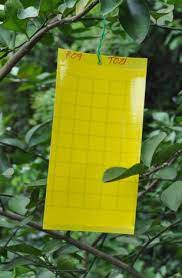
\includegraphics[width=0.3\textwidth,keepaspectratio=true]{images/C3/Trampa.jpg}
\caption{Trampa de plástico con pegamento colocada en un árbol. Imagen extraída de documentación oficial de SAGARPA}
\end{figure}


\begin{figure}[H]
\centering
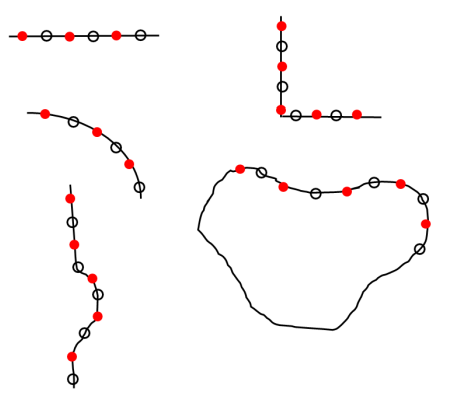
\includegraphics[width=0.5\textwidth,keepaspectratio=true]{images/Norm/ar.png}
\caption{Ejemplo de disposición de trampas en huertos irregulares. Manual operativo de la Campaña contra el Huanglongbing de los Cítrico}
\end{figure}

La distancia entre los grupos de trampas no puede superar los 700 metros, de tal forma que se cubra la totalidad de la superficie del ARCO, procurando que sus localizaciones sean equidistantes. Luego de que una trampa se coloca y el adhesivo queda expuesto, tiene una vida útil de catorce días, pues es luego de dos semanas que se retira para su monitoreo y cambio. En cada revisión, se cuentan los adultos del psílido y los datos son capturados a través del Sistema de Monitoreo de Diaphorina (SIMDIA). \textit{http://www.siafeson.com/simdia.php}.\\

\section{Métodos de control de las Campañas Mexicanas contra el HLB}

A continuación, se describen de forma particular los métodos de control usados oficialmente en las Campañas contra el HLB.

\subsection{Control Biológico en ARCOs}%IX
Existe otro tipo de control del psílido asiático de los cítricos, el control biológico, que tiene buenas implicaciones en lo que a cuidado del medio ambiente se refiere, teniendo grandes resultados en la reducción de la población de estos insectos. Las estrategias de control biológicas son utilizadas en los ARCOs conjuntamente con las sintéticas, estas estrategias son, por lo común, parasitoides y hongos entomopatógenos.\\
En las áreas especiales, como huertas abandonadas o zonas urbanas que se encuentren dentro o aledañas al control de los ARCOs, se emplea la liberación estratégica de algunos parasitoides, como Tamarixia radiata, debido a que existen algunas limitantes para el empleo de insecticidas, como riesgos de salud pública o desinterés. Las dosis que se liberan de estos parasitoides son de 100, cada 20, 50 o 100 metros, en función del grado de infestación. Existen otras estrategias, como la utilización de depredadores, por ejemplo, varias especies de Chrysoperla, o el uso de hongos entopatógenos, que causan enfermedad en el psílido, como Isaria fumosorosea o Metarhizium anisopliae, que en el laboratorio tienen niveles de mortalidad del 93.01\% de las ninfas y el 95.22\% en adultos, y en el campo mexicano reducen las poblaciones entre 48\% y 90\%.

\subsection{Eliminación de plantas}%XI

La indicación del protocolo establece que debe haber al menos cuatro monitoreos por año en los que se revise la totalidad de las plantas de cada huerta, con el fin de detectar oportunamente el HLB. Deben eliminarse de inmediato las plantas que presenten síntomas de la enfermedad cuando esta esté muy dispersa. Los recorridos para encontrar plantas con síntomas son realizados por personal capacitado, quienes marcan a las que tengan síntomas con listones, y en las plantaciones en las que la disposición sea en hileras, se marcan también las dos plantas de la hilera, que son vecinas al árbol sintomático. Posteriormente, el árbol es revisado por un técnico especializado y en caso de que el diagnóstico sea ratificado, según el protocolo: \textit{Cuando el HLB se encuentra muy disperso en el área, no se considera necesario que estas plantas sean muestreadas para proceder con la eliminación.} La poda no funciona para el control del HLB, es necesario cortar la planta y aplicar herbicida al tocón. No es necesario incinerar la planta cortada, pero sí se ha de evitar la replantación hasta que no disminuyan las poblaciones del insecto, ya que las plantas nuevas son más susceptibles, también se ha de prestar atención a los niveles de la enfermedad, puesto que no es recomendable la replantación si ésta se encuentra por encima del 5 \%.\\
En los traspatios, la responsabilidad es de los organismos auxiliares de sanidad vegetal, en contraste con lo que sucede con las huertas, en las que la responsabilidad es de los productores, quienes además promueven que no se establezcan cítricos y otros hospedantes del HLB en zonas urbanas. Lo anterior se suma a la exigencia de programas de certificación de material propagativo de cítricos, de tal forma que los viveros cuenten con mallas que impidan el paso del psílido asiático de los cítricos.


\subsection{Control Regional en huertas convencionales y huertas orgánicas}%VII
El territorio mexicano es diverso en condiciones agroecológicas y por esta razón tiene diversos escenarios epidemiológicos en lo que al HLB respecta, de modo que el control regional no es homogéneo. No obstante, el control regional se realiza en todos los casos mediante la aplicación de insecticidas, algunos foliares, que están dirigidos a los psílidos adultos pero también suprimen unos cuantos huevecillos o ninfas, además de minimizar el daño a insectos benéficos y prevenir el surgimiento de poblaciones en primavera si se aplica en invierno; por otro lado, están los insecticidas sistémicos al suelo, especialmente en plantas jóvenes como medida profiláctica. También es posible aplicar insecticida de forma extraordinaria en los focos de infección, una vez se tenga la certeza de que lo son, mediante las trampas de las que se ha hablado anteriormente en este texto. Lo deseable es que la aplicación sea en toda la región, pero si esto no es posible, la prioridad es la periferia.\\
El psílido asiático de los cítricos no es la única plaga que aqueja a los cultivos, de modo que se ha de corroborar la compatibilidad de los insecticidas, ya que algunos, como el aceite mineral, no deben mezclarse con azufre. Las aplicaciones han de ser totales, preferentemente, ya que, además de evitar contribuir al desarrollo de resistencia, también se combaten otras plagas como  el minador de los cítricos, la araña roja, o el ácaro blanco. El control regional en huertas orgánicas es especialmente importante, debido a la gran cantidad de huertos de producción orgánica y  este tipo de huerto representa un desafío especial, de modo que es necesario un plan más sólido para la zonas de producción que contengan esta mayoría de huertos. Los pulguicidas orgánicos no son eficaces en el manejo de grandes cantidades de psílidos, de modo que cuando existe un contagio mayor, es imprescindible el uso de pulguicidas convencionales, lo que hace que el huerto orgánico pierda tal calidad.


\chapter{Desarrollo experimental}
\section{Construcción de la simulación}
%CONCEPTO
%Explicar cómo se modelan, los objetos y métodos con Suposiciones y simplificaciones, hacer un resumen conceptual, no meterse en el código
En este capítulo, se describe el modelado del sistema que forman los árboles en una huerta de cítricos, el psílido vector: la Diaphorina Citri, y la bacteria: Candidatus Liberibacter. En primer lugar, el campo es visto como una cuadrícula de puntos, y en estos puntos puede o no haber un árbol; la simulación no aborda la dinámica de la enfermedad internamente en cada árbol, más bien se les ve como una unidad y cada uno tiene asociado su estado de salud y el número de psílidos que aloja; todos los psílidos   habitan en algún árbol y no abandonan el campo. En el campo, la dinámica establecida hace que los psílidos emigren a otros árboles y en su estancia en ellos corren el riesgo de infectarse si el árbol en el que están está infectado; los psílidos infecciosos se reproducen, emigran y mueren en la misma medida que los sanos; los árboles se contagian en función de la cantidad de psílidos infecciosos que alojen, y una vez infectados, se considera que son inmediatamente capaces de infectar a los psílidos que habiten en él. La unidad de tiempo de la simulación es el día, y cada árbol tiene un período asintomático que oscila aleatoriamente en torno a 200 días.
En la construcción de esta simulación se ha tratado de ser fiel a la realidad, sin embargo, el único factor de estas simulaciones que ha sido alterado respecto a lo observado, es que los psílidos se colocan aleatoriamente al centro de la huerta, y no en los bordes como lo muestra la evidencia. Esta decisión no afecta la dinámica, pero implica un enorme ahorro de recursos computacionales debido a cómo ha sido diseñado el algoritmo que sortea la migración de los psílidos.
El código puede visitarse en el siguiente repositorio:
https://github.com/HugoAceves/HLB
%Mostrar una figura de la positionsmatrix que lo ilustre

%CÓDIGO
\subsection{Los objetos del sistema}
%----------"Objetos"
%El campo
El campo es modelado como un plano conformado por una cuadrícula discreta de $n \times m$ puntos con coordenadas enteras, cualquier \textit{objeto} árbol en el campo estará solamente en algún punto de esta cuadrícula, estos puntos forman el espacio del campo, algo así como una matriz o \textit{arreglo}, todos los árboles que conformen el campo tienen las mismas características y son, en principio, sanos. A nivel del sofware, el campo es representado por varios arreglos, pero el principal es el arreglo llamado «Lista Bosque», las entradas de este arreglo son objetos de la clase árbol, y gracias a esta naturaleza, es el núcleo de la simulación; porque todos los árboles del campo están codificados en él, de tal forma que cualquier modificación que se quiera hacer en algún árbol se hace a través de la Lista Bosque. No obstante, aunque por sus características se podría decir que el campo y la Lista Bosque son lo mismo, se prefiere entender al campo como algo más que sólo la Lista Bosque. El siguiente arreglo en orden de importancia es la «Matriz Posiciones», la Matriz Posiciones es también un arreglo de $n \times m$, pero éste representa el estado de salud de los árboles, sus entradas son enteros de 0 a 4, el 0 representa que el punto está vacío, el 1 representa que en el punto hay un árbol sano y libre de psílidos, el 2 representa que en el punto hay un árbol sano que aloja psílidos, el 3 representa que en el punto hay un árbol infectado con síntomas evidentes, y a partir del 3, el arreglo no distingue si los árboles tienen o no psílidos, finalmente, el 4 representa que en el punto hay un árbol infectado y asintomático. Los dos arreglos anteriores son los que le dan soporte al campo. Hay otros tres arreglos (campo de psílido totales, campo de psílidos infecciosos, campo de psílidos sanos) que relacionan a cada punto del campo con la cantidad de psílidos que alojan, un campo refleja a los psílidos sanos, otro a los psílidos infecciosos y finalmente otro a los psílidos totales (la suma de los sanos y los infecciosos), estos arreglos han sido útiles para observar la propagación de la población del psílido con mapas de calor. Además de los arreglos, se tienen parámetros que permiten observar las estadísticas del campo a través del tiempo, tales como poblaciones de psílidos, cantidad de árboles infectados e intensidad del contagio.

%El árbol
Los árboles, como se ha dicho antes, son objetos creados para llenar los huecos del campo, éstos son vistos en su totalidad, es decir, se consideran como objetos puntuales y no se considera su dinámica interna, como el surgimiento de nuevos brotes de ramas jóvenes, las distribuciones de psílidos que haya dentro, ni si hay en ellos infección parcial. Esta consideración es útil porque simplifica la simulación sin despojarnos de lo esencial, cuando un árbol se contagia, se considera que se contagia todo, y la distribución interna de los psílidos se considera uniforme, y no se toma en cuenta su edad. Respecto al software, los atributos del objeto árbol son si está o no infectado, y las cantidades de psílidos sanos, infectados, y totales.

%El psílido y la Bacteria
El psílido es considerado en todo momento como un psílido adulto, esta simulación no se detiene en la diferencia entre los huevecillos y los cinco estadios siguientes en los que el psílido es llamado ninfa, pues aunque la evidencia muestra que los psílidos que han sido infectados desde sus estadios más jóvenes, suelen ser por lo general más infecciosos, considerar a todos los psílidos igual de infecciosos no repercute en el objeto de este trabajo. Además, se considera que todos los psílidos, una vez se contagian con la bacteria, son capaces inmediatamente de transmitirla, aunque hay que puntualizar que esto es una aproximación y no es lo real. Tampoco se parte de que haya diferencias de ningún tipo entre el comportamiento de los psílidos portadores de la bacteria y los sanos, esto implica particularmente que su migración y su mortalidad es la misma. Respecto al software, el psílido no es modelado como un objeto, es, más bien, un parámetro de cada árbol, esto implica que no existe un seguimiento particular de los individuos, sino que son más bien una cantidad, y su comportamiento es estudiado de una forma «macroscópica»; esto tiene notables ventajas si se toma en cuenta que las poblaciones de Diaphorina Citri en un huerto común pueden ser de cientos de miles. La bacteria en esta simulación corre una suerte similar a la del psílido, pues en realidad no aportaría demasiado concebirla de algún modo especial, dado que su comportamiento en lo colectivo es estable, esto es, que los psílidos la adquieren de los árboles y los árboles de los psílidos de forma monótona, sin mencionar el evidente hecho de que su modelado individual es imposible para los recursos de este experimento.

\subsection{Las relaciones entre los objetos del sistema}
%----------"Métodos"
%Fill_field
Se ha hablado suficiente de los objetos del sistema, de modo que lo siguiente es abordar el comportamiento y las relaciones que hay entre ellos. Una vez que se ha creado el arreglo del campo, este está vacío, así que es llenado por los objetos árbol dejando algunos huecos aleatoriamente; posteriormente se pone en funcionamiento la dinámica, cuya unidad de tiempo es el día, por cada día se ejecuta un ciclo de actualización que está constituido por cuatro partes: la propagación de los psílidos a otros árboles, su reproducción, la infección de los árboles a través del vector, y la infección de algunos de los psílidos que habiten árboles infectados. Antes de comenzar la simulación, se colocan aleatoriamente psílidos en algún árbol arbitrario, la cantidad de psílidos benignos e infecciosos se determina como más convenga al momento de ejecutar la simulación.

%Spread
La difusión del psílido es una de las partes más elaboradas del código de esta simulación. Antes de iniciar la simulación, se ingresa un parámetro que se entiende como la «intensidad» con la que los insectos emigran a otros árboles, esta intensidad es dada según convenga por quien ejecute la simulación, y es un número entre cero y uno. La primera parte de la difusión comienza con la elección de los árboles de los que saldrán los psílidos migrantes, el número de árboles a elegir es una fracción de los árboles que alojen psílidos en ese momento, esta fracción está dada justamente por el parámetro «intensidad» multiplicado por la cantidad de árboles con psílidos. Si se diera el caso en el que esta cantidad de árboles con psílidos fuera muy pequeña, el producto (o cociente, dado que $0<intensidad<1$), podría ser menor que uno; lo que implicaría que ningún árbol estaría disponible para enviar sus psílidos a otros, algo que se evita eligiendo siempre al menos un árbol para que emigren psílidos desde él, pues, de otro modo, los psílidos se quedarían siempre en el mismo árbol desde el principio de la simulación. Ya que se tiene la cantidad de árboles a elegir, éstos se eligen aleatoriamente, con la natural condición de que en efecto alojen psílidos y de que un mismo árbol no se elija más de una vez por ciclo.
Una vez se tiene una lista con los árboles que serán el origen de la migración, se elige, a un árbol destino para cada uno de estos árboles origen. Los árboles destino que se asocian a los árboles origen son elegidos mediante dos criterios, el espacial, y el relativo a la proporción de psílidos que haya entre ellos. Sea $n$ la altura del campo y $m$ el ancho. El primer paso para elegir al árbol destino es el espacial, se toma primero la posición del árbol origen, que es una pareja de la forma $(x, y)$, con $x, y \in \mathbb{N}$ que cumplen naturalmente que $x\leq m,$ $ y \leq n$, posteriormente a esta pareja se le suma otra pareja aleatoria $(a, b)$, de este modo, la posición del árbol destino será $(x+a, y+b)$. Es fácil notar que la elección de $a$ y de $b$, determina en gran medida la dinámica de los psílidos a través de la huerta, en este modelo, en lugar de simular que los psílidos viajan solamente a los árboles contiguos (esto es $a, b \in \{1, 0, -1\}$), se prefirió, en primer lugar, tener en cuenta el patrón de sembrado, y en segundo lugar permitir que los psílidos viajasen a otros árboles más lejanos. El patrón de sembrado tiene que ver con el hecho de que en las huertas reales, los árboles no suelen estar sembrados en una cuadrícula, pues resulta muy útil disponerlos en largas columnas con cierta separación entre sí, de tal forma que esto permita el desplazamiento de maquinaria y recolectores entre ellas, así que aunque se simula el campo como una cuadrícula, el desplazamiento de un psílido está condicionado por esta característica, verticalmente $(0, y)$ (a lo largo de una columna) la distancia recorrida suele ser mucho más probable y amplia que la horizontal $(x, 0)$ (entre columnas), puesto que para estos insectos los árboles de la misma columna quedan más cerca que los de otras columnas. Los valores de desplazamiento, se sortean con una distribución de probabilidad binomial centrada en el cero, esto implica que el desplazamiento en cada dimensión, será un número entero, con el cero siendo el valor más probable, el 1 y el -1 los segundos más probables, el 2 y el -2 los terceros más probables, y así sucesivamente. Está claro que en esta situación, la pareja de desplazamiento más probable será $(0, 0)$, sin embargo, cuando esto sucede, la simulación descarta ese valor y vuelve a sortear, en virtud de que lo que se busca es que el psílido emigre, y esta pareja implicaría que el psílido se «mude» al propio árbol en el que habita. El desplazamiento típico suele ser unitario en alguna de las cuatro direcciones, o diagonal con la forma $(1, 1)$, aunque en última instancia, todos los desplazamientos son posibles. Finalmente, ya que se tiene la posición del árbol destino, entra en juego el segundo criterio; el de la proporción de psílidos. Sería posible que en estas condiciones se mudaran los psílidos al árbol elegido previamente, sin embargo, pudiera darse el caso en el que este árbol destino alojara ya demasiados psílidos, más incluso que el árbol origen desde el que parten los insectos, de modo que no sería razonable, que éstos abandonasen la posición que habitan para llegar a una donde hubiese más insectos aún, puesto que se parte de la suposición de que la migración es consecuencia de la búsqueda de posiciones con más recursos disponibles, así que si la cantidad de psílidos en el árbol destino es mayor que la del árbol origen, los psílidos simplemente no emigran y se sortea de nuevo una posición. Si se da el caso inverso, en el que la proporción de psílidos en el árbol destino sea menor que la del árbol origen, entonces se sortea la migración de los psílidos en función de esta proporción; cuanto más cercana sea esta proporción a 1 (esto es, que las cantidades de psílidos en ambos árboles son casi iguales) menos probabilidad hay de una mudanza, mientras que cuanto más cercana sea la proporción a 0 (esto es, que la cantidad de psílidos en el árbol origen es mucho mayor que la del árbol destino) más probable es que los insectos emigren.
%PONER FIGURA DE PATRÓN DE SEMBRADO AQUÍ


%update_diaphorina_amount
A pesar de que en esta simulación no se considera el proceso de reproducción y crecimiento del psílido, constituido por la etapa de depósito de huevecillos en los brotes tiernos de los árboles y los cinco posteriores estados en los que es una ninfa, es necesario considerar que la población de psílidos crezca, esto se hace mediante una ecuación logística caracterizada con la cantidad máxima observada experimentalmente de 30 mil a 40 mil psílidos por árbol. No se considera que los psílidos infectados tengan diferencia alguna con los no infectados respecto a su natalidad y mortalidad, de modo que a cada actualización de la simulación, la multiplicación de estos dos tipos de psílido es proporcional entre sí y congruente con la ecuación logística.
%PONER LA ECUACIÓN CARACTERIZADA AQUÍ (Y TAL VEZ UNA GRÁFICA DE LA DINÁMICA)
%Incluir referencia que respalde el dato de los psílidos por árbol marcada con el número 25 e el artikel

%Update_infected trees
Luego de que se han multiplicado los psílidos, se continúa con la infección de los árboles que adquieren la bacteria que portan los psílidos infecciosos que alojen, la infección de estos árboles obedece la distribución de probabilidad dada por $ \frac{n^2}{c+n^2}$, donde $c$ es una constante y $n$ es la cantidad de psílidos infecciosos que haya en el árbol. Dado que uno de los principales intereses de este trabajo yace en la infección asintomática, esta parte de la simulación es fundamental. Cuando un árbol es sorteado como infectado, se considera inmediatamente infeccioso debido a que esto es una aproximación bastante realista, puesto que experimentalmente existe evidencia de que el período que tarda un árbol en tornarse infeccioso (período de latencia) no rebasa los quince días, esto es, que la bacteria ya habita en el árbol pero no de una forma tal que el árbol esté en condiciones de infectar a los psílidos que habiten en él; esta aproximación es útil para simplificar el modelo sin perder precisión. Respecto al periodo de incubación, que es el tiempo que tarda un árbol en mostrar  los síntomas, se parte de la evidencia que sugiere que los árboles tardan en promedio 200 días en presentar síntomas, aunque en este trabajo se usen también otros tiempos de incubación. Cuando un árbol es sorteado como infectado, se le asigna algún período de incubación aleatorio en una vecindad en torno a 200 días; el tamaño de la vecindad es determinado al iniciar la simulación. Cuando los árboles cumplen el período de incubación asignado, pasan de ser asintomáticos a ser simplemente árboles infectados.
%Profundizar en la probabilidad de infección
%Poner referencias que justifiquen los 15 días de infección (25 EN ARTIKEL)y 200 días asintomáticos (1 EN ARTIKEL)

%Update_infected diaphorina
Al final de este proceso, y una vez que los nuevos árboles han sido infectados, una fracción de los psílidos sanos que habiten en un árbol infectado se infectan, esto sucede sin importar si el árbol es asintomático o no. Cuando esta parte de la simulación termina, se considera que ha concluido un ciclo, que equivale al paso de un día en una huerta real. La cantidad de ciclos es determinada al inicio de cada simulación y su transcurso implica que los cambios en las propiedades de la huerta se muestren en función de los días transcurridos.

\subsection{Los métodos de control}
%----------"Métodos de control"
%Fumigación
Los métodos de control simulados en este trabajo son descritos con mayor detalle en el capítulo anterior, estos métodos son contemplados por la normatividad oficial en México. El primer método de control es el de la aplicación periódica de pesticidas o algún agente que reduzca la población de psílidos. Más allá de los mecanismos químicos y biológicos mediante los cuales estos agentes logran su cometido, la simulación se centra exclusivamente en su efecto sobre la cantidad de insectos que habitan los árboles de la huerta. A un nivel general, estos agentes no tienen un efecto notable en la distribución de los psílidos debido a que se aplican uniformemente en todos los árboles, pero sí influyen notablemente en reducir el número de psílidos que los habitan, de modo que, para los efectos de estos experimentos, la aplicación de pesticidas o agentes similares se reduce a eliminar una fracción constante de los insectos de cada árbol, esta fracción varía según el método empleado y factores ambientales. Esta simulación está diseñada de tal forma que la frecuencia de aplicación de los pesticidas y su potencia pueden variarse según el escenario que se busque estudiar, la frecuencia está medida en días y la potencia es el porcentaje de psílidos que el pesticida elimina luego de su aplicación. Este método no discrimina entre psílidos infecciosos y sanos, ni factores climáticos, y su efecto es puntual en el tiempo.

%Corte
Otro método probado en esta simulación es el de vigilar periódicamente cada árbol de la huerta a fin de detectar a los árboles que sean portadores de la enfermedad y talarlos, para evitar que propaguen la bacteria a más psílidos y con esto la enfermedad se difunda dentro de la huerta. Aunque, en algunos casos, los productores prefieren asegurarse mediante pruebas de laboratorio que los árboles con síntomas están en efecto contagiados con HLB, la recomendación indica que, cuando la cantidad de contagios es alta, los árboles con síntomas deben ser cortados inmediatamente\cite{robles2012protocolo}. El cerciorarse de que los síntomas se deban a HLB y no a otros factores ayuda a no deshacerse de árboles sanos por error, pero implica también la demora de varios días desde que se detectan los síntomas hasta que se tiene una confirmación por laboratorio, de modo que si el árbol fuera portador de la bacteria, se estaría actuando con retraso. Es por lo anterior que en este modelo se toman en cuenta diversos escenarios de control, unos en los que la vigilancia es más rigurosa y la tala inmediata, y otros en los que la vigilancia es más laxa. Finalmente, el protocolo indica que ante la detección de un árbol sintomático y su tala, se ha de eliminar previamente a los psílidos que habiten en él, de modo que en esta simulación los psílidos son eliminados junto con el árbol que habitan. Dicho lo anterior, es importante puntualizar que en esta simulación no se ha considerado que existan falsos positivos porque este efecto no condiciona directamente el objeto de interés.

%Corte de vecinos
Una medida extra de seguridad es la de talar no solamente el árbol con síntomas, sino a sus árboles vecinos. Esta medida contempla claramente el efecto asintomático, dando importancia al hecho de que existe cierta probabilidad de que si un árbol está infectado, los árboles que lo rodean estén también infectados aunque aún no muestren síntomas. El protocolo indica ciertos criterios para decidir la viabilidad de la tala de los vecinos, estos criterios se basan en la proporción de árboles infectados detectados en la zona y la cantidad de psílidos que habiten en los árboles. En algunos casos, es recomendable hacer una revisión de laboratorio a los árboles contiguos mientras que en los casos de mayor infestación es preferible talarlos directamente. Finalmente, se entiende por «vecinos» a los cuatro árboles adyacentes, en dirección norte, sur, este y oeste, sin contar a los árboles que estén en alguna diagonal, por ejemplo noroeste.

%----------

\section{Ejecuciones del código}
%Exordium
El código del programa que simula al sistema se ha ejecutado varias veces, cada una modificando algunas variables. En esta sección se habla de las cantidades que se variaron y el porqué, además de las cantidades que se mantuvieron constantes para todas las simulaciones.

\subsection{Variables características}
La primer variable característica que se ha determinado es el tamaño del campo, que en principio no debería suponer un cambio sustancial en el comportamiento dinámico del sistema; para esta variable se ha elegido un campo de 49 filas por 62 columnas, esta elección ha estado basada en un campo real en el estado de Tamaulipas (Figura 4.1).\\
\begin{figure}[H]
\centering
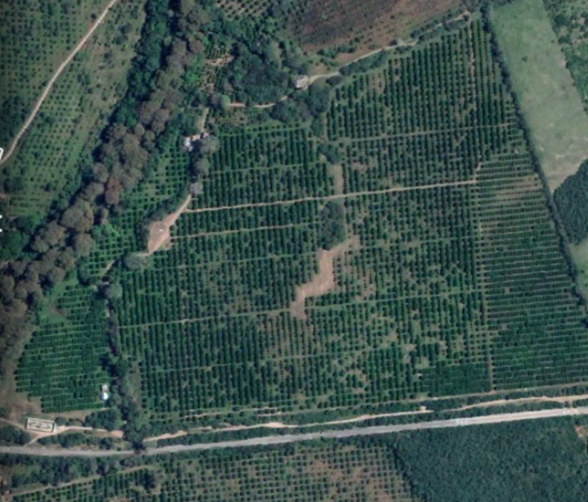
\includegraphics[width=0.5\textwidth,keepaspectratio=true]{images/C4/Huerta.png}
\caption{Plano cenital de una huerta en el estado de Tamaulipas.}
\end{figure}
La posición inicial de los psílidos no está basada en las observaciones de campo, pues comúnmente cuando éstos llegan a poblar un campo, se instalan en los árboles de los extremos de la huerta y difícilmente arriban a árboles más céntricos, sin embargo, como en este trabajo se resume el problema a una sola huerta, este hecho no tiene un efecto relevante, y el comportamiento de la enfermedad se torna más perceptible cuando más al centro se coloquen inicialmente los psílidos. Una vez colocados en algún punto aleatorio del campo, la distancia que suelen recorrer los psílidos en un día no rebasa algunos cuantos metros; cabe mencionar que los efectos del viento en la dinámica del insecto no ha sido considerada en este trabajo. La cantidad inicial que es colocada es arbitrariamente de 100 individuos, de los cuales el 15\% está infectado, su crecimiento se ha modelado por la función logística con una capacidad máxima en cada árbol de 300 centenas de insectos, esta capacidad máxima ha sido observada en campos en los que no se aplica control de la plaga. En el caso de esta simulación, dadas las dimensiones del campo y la capacidad máxima de cada árbol, la capacidad total de la huerta está por encima de las novecientas mil centenas. La probabilidad de contagio de un psílido que se alimenta del árbol, así como la probabilidad de transmisión de la bacteria en los psílidos infectados a los árboles sanos han sido calibradas para reproducir los niveles observados de árboles sintomáticos a través del tiempo. El tiempo de incubación se ha configurado para ser en promedio de 200 días, esta cantidad ha sido observada para al menos una especie de cítrico, y los valores se desvían de esta cantidad dentro de un entorno de ±50 días, aunque para algunos experimentos fueron probados entornos de distinto radio.

\begin{table}[!ht]
    \centering
    \begin{tabular}{|l|p{0.7in}|p{0.7in}|p{0.6in}|p{0.7in}|p{0.65in}|p{0.45in}|}
    \hline
        Nombre & Tiempo de \newline incubación\newline mínimo & Tiempo de\newline incubación\newline máximo & Per'ioodo\newline del\newline pesticida & Mortalidad\newline del\newline pesticida & Periodo de\newline revisión\newline y corte & Corte\newline de\newline vecinos  \\ \hline
        Control1 & 150 días & 250 días& Ninguno & Ninguno & Ninguno & No  \\ \hline
        Control2 & 165 días & 235 días& Ninguno & Ninguno & Ninguno & No  \\ \hline
        Control3 & 180 días& 220 días& Ninguno & Ninguno & Ninguno & No  \\ \hline
        Pesticida1 & 150 días& 250 días& 90 días& 50\%& Ninguno & No  \\ \hline
        Pesticida2 & 150 días& 250 días& 90 días& 70\%& Ninguno & No  \\ \hline
        Pesticida3 & 150 días& 250 días& 90 días& 90\%& Ninguno & No  \\ \hline
        Pesticida4 & 150 días& 250 días& 60 días& 70\%& Ninguno & No  \\ \hline
        Pesticida5 & 150 días& 250 días& 90 días& 70\%& Ninguno & No  \\ \hline
        Pesticida6 & 150días & 250 días& 180 días& 70\%& Ninguno & No  \\ \hline
        Corte1 & 150 días& 250 días& Ninguno & 70\%& 90 días& No  \\ \hline
        Corte2 & 150 días& 250 días& Ninguno & 90\%& 60 días& No  \\ \hline
        Corte3 & 150 días& 250 días& Ninguno & 70\%& 15 días& No  \\ \hline
        CorteVecinos & 150 días& 250 días & 90 días& 70\%& 90 días& Sí  \\ \hline
        PesticidaCorte & 150 días& 250 días& 90 días& 70\%& 90 días& Sí  \\ \hline
    \end{tabular}
\end{table}


\subsection{Pruebas principales con distintas variables}

%--------------------------------------------------------------------------------HORNADA PRINCIPAL

%Simulación de control
%Pesticida solo
%Corte individual
%Corte Vecinos
%Métodos conjuntos

La primera ejecución del código tiene el objetivo de servir como punto de referencia para las simulaciones próximas, por esta razón, los métodos de control han sido omitidos de tal forma que la plaga y la enfermedad puedan desarrollarse libremente. En esta y en las siguientes simulaciones, el tiempo medio de aparición de síntomas en árboles infectados es de 200 días a partir de su infección, este período de incubación puede tomar valores mínimos de 150 días y máximos de 250.
La segunda ejecución contempla el mismo escenario que la ejecución de control pero adhiere la aplicación periódica de pesticida cada noventa días, aproximadamente tres meses, que es el tiempo mínimo indicado por el protocolo. La mortalidad en la aplicación es del 70\%, que es el valor medio de la medida en los experimentos de campo, y es consistente con la información proporcionada por los fabricantes. La aplicación de pesticida es el único método de control de esta simulación.
La tercera ejecución, por otra parte, usa el método de control que consiste en una revisión periódica de todos los árboles de la huerta cada 60 días y el corte inmediato de los árboles que presenten síntomas de infección, este método es el único que se aplica en la tercera ejecución.
La cuarta ejecución es idéntica a la tercera salvo por el criterio para cortar árboles, dado que mientras que la tercera solamente corta al árbol con síntomas, en esta se talan también a los cuatro árboles contiguos al árbol sintomático.
Finalmente, las simulaciones quinta y sexta combinan los métodos usados en las simulaciones cuarta y segunda, con la diferencia de que en la simulación quinta el tiempo de revisión para tala es de noventa días mientras que en la sexta es de 15. Los métodos usados son una representación fiel de lo que se practica en los campos reales, el control en la población de psílidos y la eliminación de los árboles infectados y sus vecinos junto con los psílidos que contengan. Los resultados que retornaron son útiles para entenderlos.


%--------------------------------------------------------------------------------HORNADAS SECUNDARIAS SI SE NECESITASEN
%\subsection{Pruebas secundarias con distintas variables}
%Pruebas de control

%Aplicación de pesticidas sin tala
%Dureza del pesticida(50%, 70%, 90%)a 3 meses

%Período del pesticida(6meses, 3 meses, 2 meses)con el 70%

%Tala de árboles sin pesticidas
%   Individual
%Tiempo de vigilancia(90, 60 y 15 días)

%   Con vecinos
%a 90 días

%Métodos de control conjunto
%3 meses 70%
\chapter{Resultados y análisis}


%Simulación de control
%Pesticida solo
%Corte individual
%Corte Vecinos
%Métodos conjuntos
En este capítulo se describen los resultados encontrados en este trabajo y su interpretación. La cantidad de información arrojada por las ejecuciones del código descritas en el capítulo anterior es amplia, y será analizada a continuación.

\section{Comparación de la dinámica de crecimiento de árboles asintomáticos usando distintos métodos de control}
%Códigos 1, 2 y 3: Gráfica de asintomáticos --------------------------------------------------------------------------------------------------------------------------------COMPARACIÓN DE MÉTODOS
Uno de los intereses de este trabajo ha sido el de observar el comportamiento de los métodos usados en el campo mexicano para reducir la propagación de la enfermedad. Los métodos de especial interés son la reducción directa y periódica de la población de psílidos, y la eliminación de los árboles con síntomas. A continuación, se muestra la evolución temporal de las poblaciones en una huerta en condiciones normales\cite{dala2019effect} \cite{robles2012protocolo}.
\begin{figure}[H]
\centering
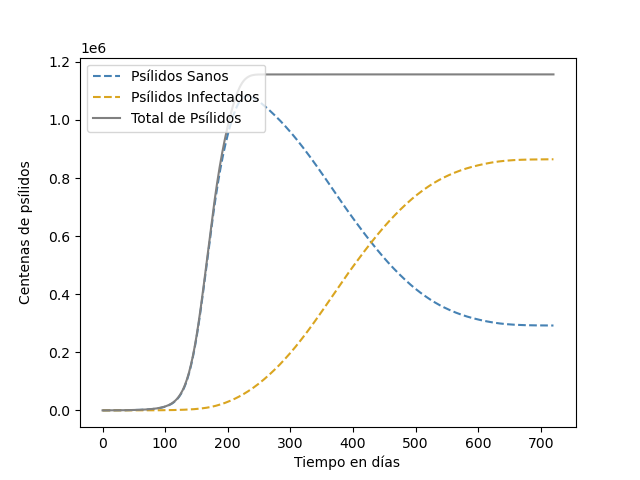
\includegraphics[width=0.7\textwidth,keepaspectratio=true]{images/Imágenes C6/C6-0.png}
\caption{Crecimiento de las poblaciones de psílidos infecciosos, sanos y totales en un campo sin ningún método de control.}
\end{figure}
%Hechos:
%PRIMERO: La aplicación de pesticidas es la mejor herramienta para combatir la enfermedad si no se tiene acceso a información sobre árboles asintomáticos, es buena incluso sin el corte de los árboles
La primera observación que se ha desprendido de las simulaciones en las que se compararon los métodos de control, es que la aplicación de pesticidas o algún agente que reduzca en general a la población, es la mejor herramienta para combatir el crecimiento de la enfermedad dentro de la huerta. Especialmente si no se tiene acceso a ninguna clase de información sobre la cantidad y ubicación de los árboles asintomáticos y los infectados, llegando a ser buena incluso sin el corte de los árboles sintomáticos. A continuación, se muestran tres gráficas distintas que representan a la matriz de posiciones, cada una generada por la ejecución del código con distintos métodos de control.
\begin{figure}[H]
\centering
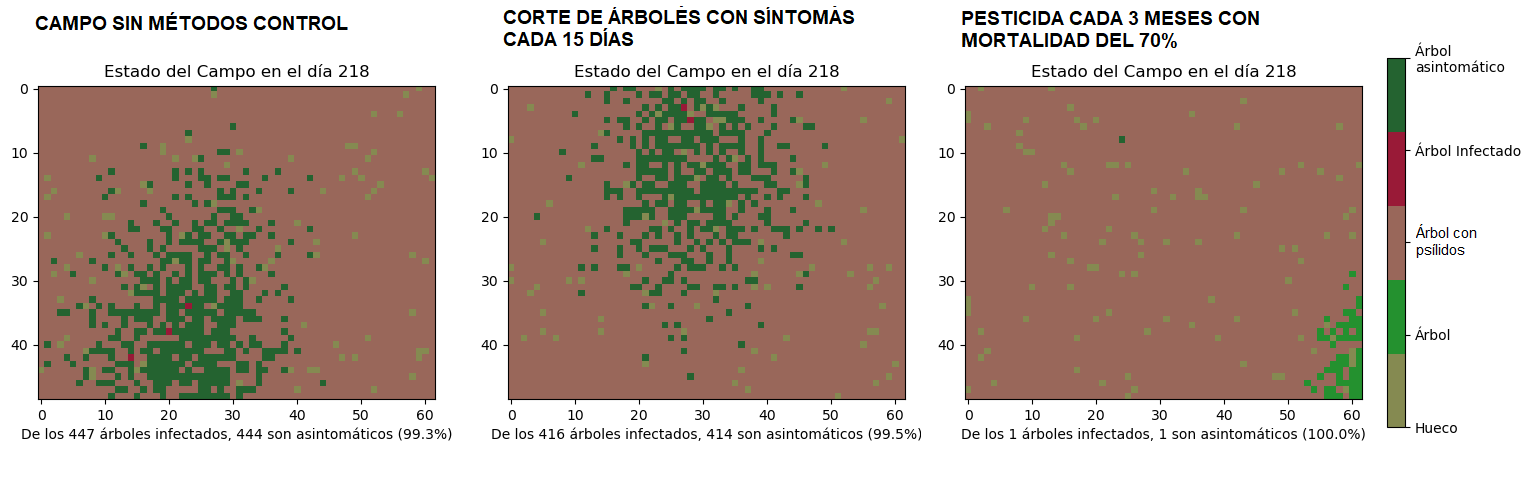
\includegraphics[width=1\textwidth,keepaspectratio=true]{images/Imágenes C6/C6-1.png}
\caption{Comparación del estado tres campos con distintos métodos de control luego de 218 días de haber sido inoculado con psílidos infecciosos}
\end{figure}
De lo anterior, se puede observar la importancia que tiene la aplicación de pesticidas de forma periódica y su contraste con métodos que prescinden de ella. Como se puede observar, cuando las medidas de control son endebles, la propagación asintomática es veloz, y mientras que para el momento en el que las huertas con control pesticida comienzan a infectarse, en las huertas sin pesticidas la infección ya tiene un avance significativo. También se puede observar que la tala de los árboles sintomáticos aporta algo de control a propagación, pero este esfuerzo es insuficiente. 

%SEGUNDO; La acción combinada de los anteriores métodos retrasó en promedio la aparición de árboles sintomáticos hasta los 260 días

Otra faceta explorada en este trabajo es la del control conjunto y coordinado de los dos métodos anteriores, en ella se encontró que su acción combinada retrasó la aparición de árboles sintomáticos hasta los 260 días en promedio. Y quedó en evidencia el resultado predecible de que cuanto más campañas de aplicación de pesticidas haya, menos se esparce la bacteria a través de los árboles de la huerta. A continuación, se muestran dos campos en los que el período de revisión de síntomas es de quince días y el periodo de aplicación de pesticidas es de dos meses y quince días respectivamente, representando este último un caso extremo. Cada campo es mostrado en el día en el que han aparecido los primeros árboles con síntomas.
\begin{figure}[H]
\centering
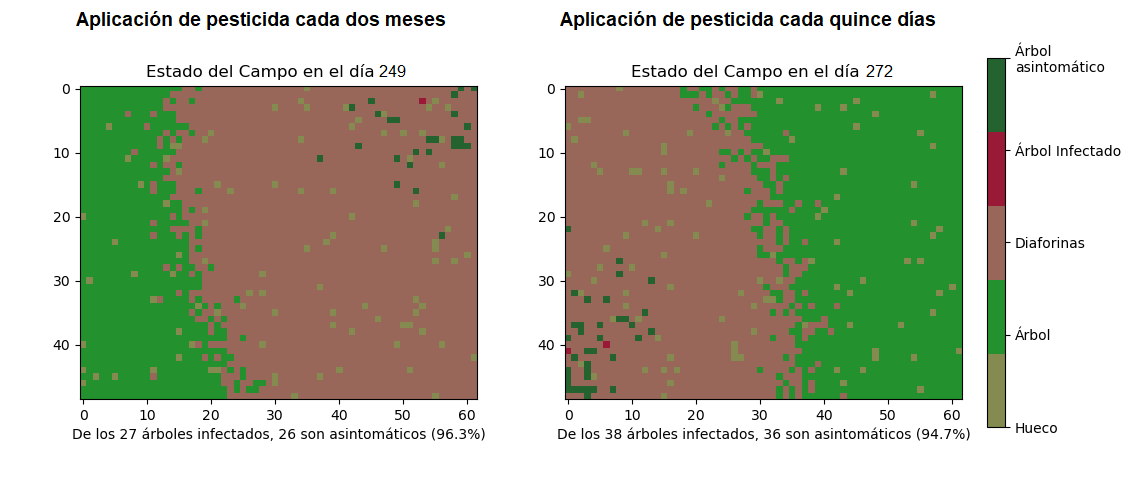
\includegraphics[width=1\textwidth,keepaspectratio=true]{images/Imágenes C6/C6-2.png}
\caption{Comparación del estado dos campos en los que se aplica pesticida con diferentes períodos, luego de 218 días.}
\end{figure}

%TERCERO: Aunque los métodos combinados, no redujeron a cero la población de psílidos, tuvieron un impacto mayor en la población de psílidos infecciosos y esto parece tener implicaciones directas en la cantidad de árboles infectados

De lo anterior, queda claro que aunque este método de control reduce notablemente la población de psílidos, no la elimina del todo, sin embargo esto no evita que tenga un impacto considerable en la población de psílidos infecciosos. Se ha visto recurrentemente en las simulaciones de este trabajo que hay una fuerte relación entre las regiones con gran presencia de árboles infectados y las regiones con gran presencia de psílidos infecciosos, de tal forma que en la mayoría de los casos, estas regiones suelen ser casi idénticas, y esto parece tener implicaciones directas en la cantidad de árboles infectados, y esto podría ser un indicio de que tener datos fiables de la distribución y cantidad de psílidos infecciosos en una huerta, conduciría irremisiblemente a estar en condiciones de inferir la región de árboles asintomáticos.

%CUARTO: El efecto de cortar los árboles vecinos es despreciable
En esta simulación, también se valoró la viabilidad de talar a los árboles vecinos de un árbol detectado como infectado, sin embargo su impacto en la reducción de la enfermedad fue despreciable, y su repercusión en la reducción de la cantidad de árboles de la huerta fue grande.
	
%Conclusión: 
En síntesis, la efectividad de los métodos estudiados se ha puesto de manifiesto, además de la evidencia de que estos métodos conjuntos son aún más efectivos. También se ha visto que el problema de combatir la propagación de HLB se puede ceñir de buena forma al combate exclusivo de los psílidos infecciosos, de modo que conocer la distribución de estos dentro de la huerta es una herramienta útil para inferir la distribución de árboles asintomáticos dentro de ella.


%Códigos 1, 3, 4, 5 y 6: Gráfica de Distribución de psílidos y gráfica de distribución de asintomáticos ---------------------------------------------------------------------DINÁMICA DE LOS PSÍLIDOS INFECCIOSOS
\section{Dinámica de los psílidos infecciosos}
%Hechos: 
%PRIMERO: La distribución de psílidos infecciosos y sanos no es igual, pese a que sus patrones de movimiento son iguales, los árboles infectados son los que alojan a la gran mayoría de psílidos ifectados. 
Uno de los principales resultados, respecto a la dinámica de los psílidos, ha sido que la distribución de psílidos infecciosos no es igual a la de los sanos pese a que sus reglas de movimiento son iguales dentro del código de la simulación, y en todas las simulaciones se ha observado que los árboles infectados son los que alojan a la gran mayoría de psílidos infecciosos, como se ha dicho antes. A continuación, en la Figura 5.4, se muestran las distribuciones de psílidos dentro de una huerta. El primer cuadro corresponde a la \textit{matriz de posiciones} y los tres restantes corresponden a los \textit{campos de psílidos} descritos en el capítulo 4, se ha tomado el día 134 porque en él se ha notado el mayor contraste.
\begin{figure}[H]
\centering
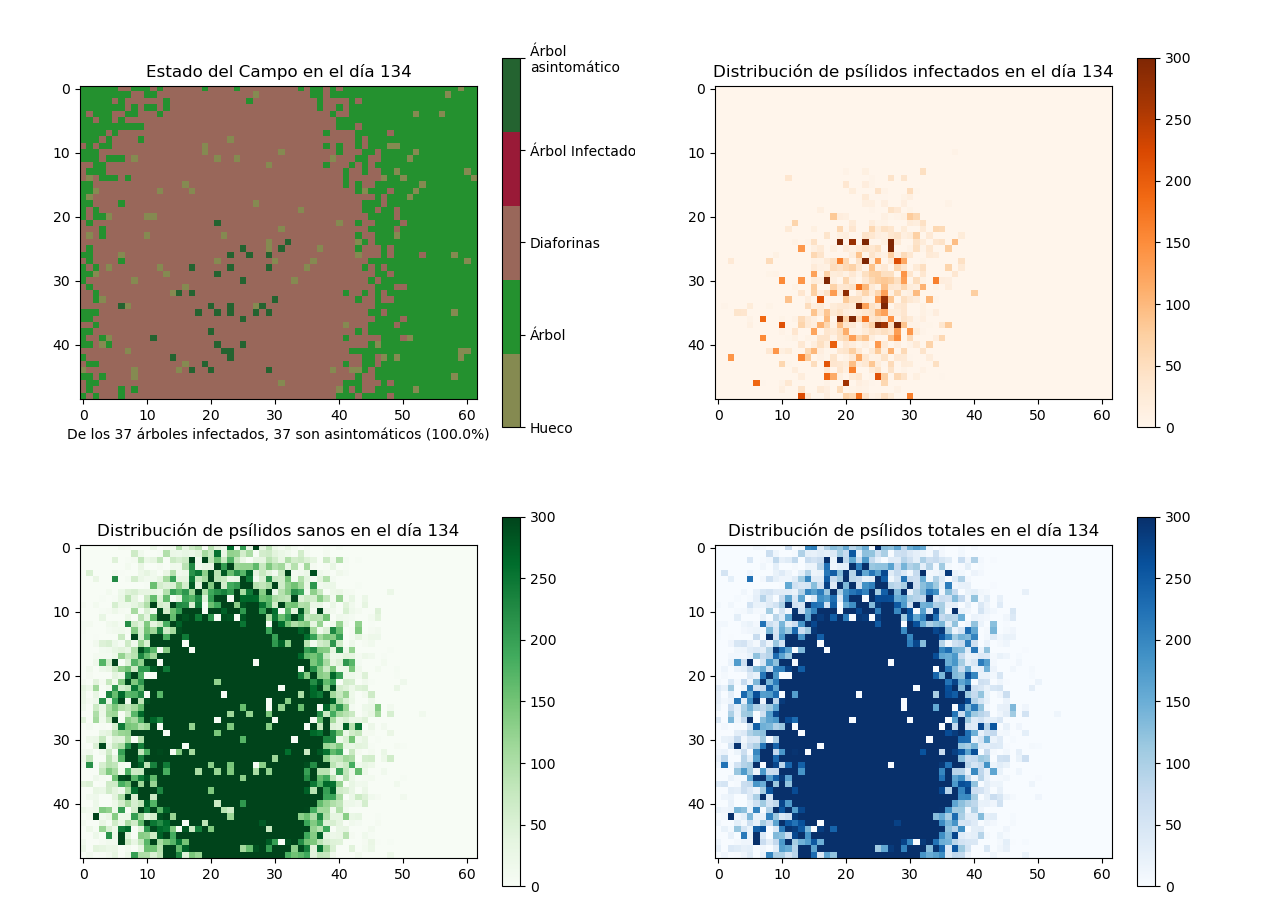
\includegraphics[width=1.\textwidth,keepaspectratio=true]{images/Imágenes C6/C6-3.png}
\caption{Estado del un campo sin control luego de 134 días de haber sido inoculado con psílidos infecciosos. }
\end{figure}
En la figura anterior, el cuadro superior izquierdo muestra la distribución de árboles asintomáticos y sanos, el resto de cuadros muestran la concentración de psílidos clasificados, en ella puede observar que la distribución de los psílidos sanos prácticamente se ajusta a la de los psílidos totales en el campo, esto se puede ver como que las zonas con presencia de psílidos tienen por lo general al menos algo de presencia de psílidos sanos, sin embargo, esto no sucede igual con los psílidos infecciosos, que están por lo general en las mismas zonas donde hay presencia de árboles infectados, ya sean estos asintomáticos o no.
La figura anterior muestra una huerta sin ningún método de control, pero todas las huertas simuladas tienen esta característica, además de que tienden a la eventual infección de todos sus árboles y a ser ocupadas por psílidos infecciosos. El crecimiento de las regiones de psílidos infecciosos sigue al crecimiento del total de psílidos.

%SEGUNDO: Hay incluso algunos huertos, donde la infección es tan fuerte, que en los lugares con psílidos infecciosos hay gran ausencia de psílidos sanos.
Se ha observado también que cuando la infección es suficientemente fuerte en algún huerto, en las zonas con psílidos infecciosos hay una gran ausencia de psílidos sanos. La explicación que se propone es que esto es una consecuencia de que la zona y su entorno han alcanzado el máximo de población de psílidos que puede alojar, de modo que los psílidos difícilmente emigran y la población no se renueva, y esto, sumado al largo tiempo en el que el árbol ha sido transmisor de la bacteria, provoca que la mayoría de psílidos dejen de ser sanos para convertirse en infecciosos. Esta propuesta es congruente con el hecho observado de que los psílidos que emergen de los huevecillos depositados en árboles infectados, suelen portar concentraciones más altas de la bacteria, y así, los psílidos sanos terminan por morir o por infectarse.
Este efecto podría ser también una forma de detectar indirectamente las zonas con mayor presencia y longevidad de árboles infectados; se podrá deducir que cuanto menor sea la fracción de psílidos sanos en alguna zona, la enfermedad en esa zona es más intensa. Esto tiene la evidente ventaja de que la medición se convierte en un asunto de proporción y no de cantidad, siendo esta una vía más factible para los agricultores. Si se toma una muestra de cierta cantidad representativa de los psílidos que habitan un punto de la huerta, y se cuenta la cantidad de psílidos sanos, se estaría en condiciones de estimar la intensidad de la enfermedad en ese punto. Este efecto se ilustra a continuación, en la figura 5.5:
\begin{figure}[H]
\centering
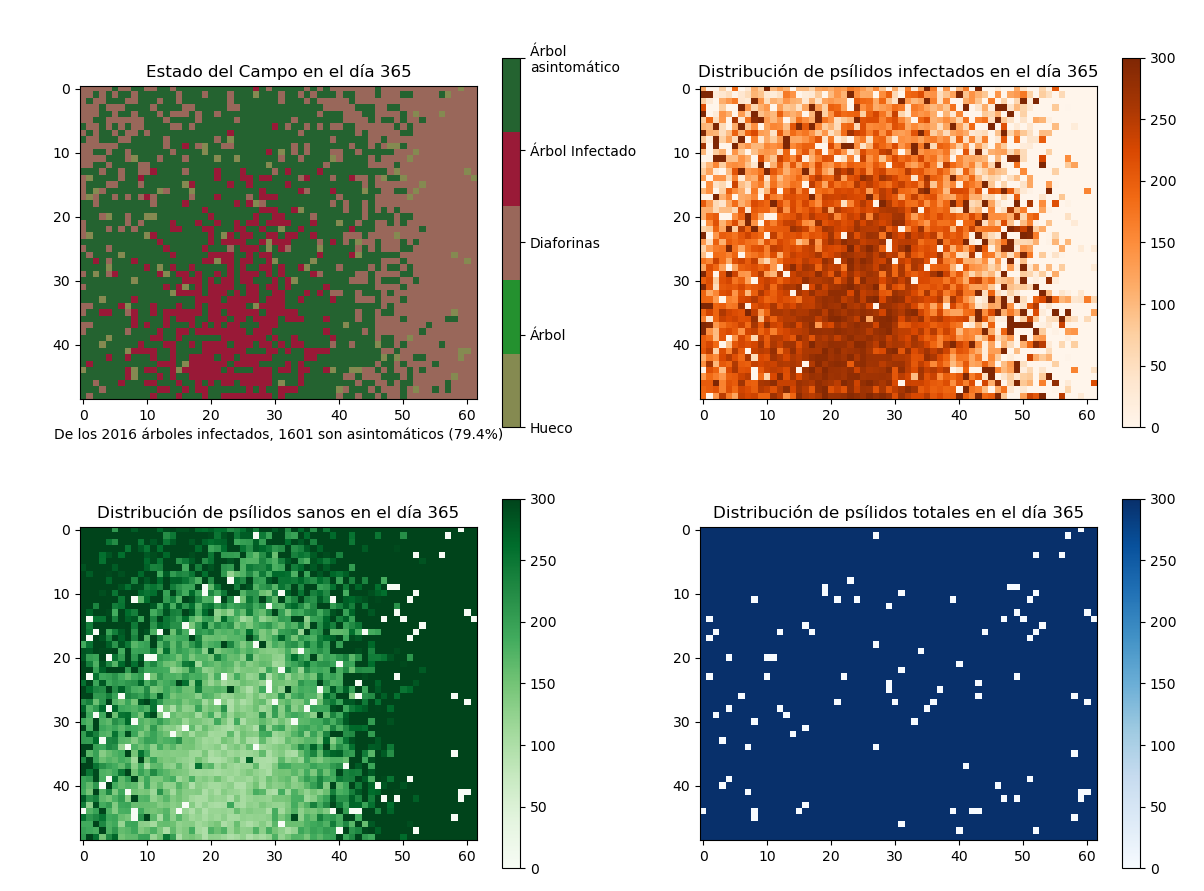
\includegraphics[width=1.\textwidth,keepaspectratio=true]{images/Imágenes C6/C6-4.png}
\caption{Estado del un campo sin control luego de un año. La ausencia de psílidos sanos es notable en las zonas con más árboles sintomáticos.}
\end{figure}

%TERCERO: La distribución de población de psílidos infecciosos es una mancha
Algo que se aprecia en todos los mapas de distribución de los psílidos, sin importar incluso si se usan métodos de control, es que suelen ser manchas ligeramente ovaladas verticalmente, con un centro normalmente cercano al lugar donde los psílidos fueron inicialmente depositados, y cuyo radio crece a través del tiempo. Este hecho implica que la zona de riesgo de contagio está acotada por alguna distancia que dependa del tiempo transcurrido. Sería de interés para estudios futuros el investigar la relación que existe entre la proporción de psílidos infecciosos en alguna zona, y el radio de la zona de psílidos infecciosos.

%CUARTO:La población de psílidos forma además una especie de onda 
La última observación de interés en cuanto a la dinámica de los psílidos infecciosos es la presencia de un «patrón de ondas» generado en las huertas en las que hubo aplicación de pesticidas periódicamente. Hasta ahora no se tiene ninguna hipótesis a este respecto, un ejemplo se muestra a continuación, en la figura 5.6:
\begin{figure}[H]
\centering
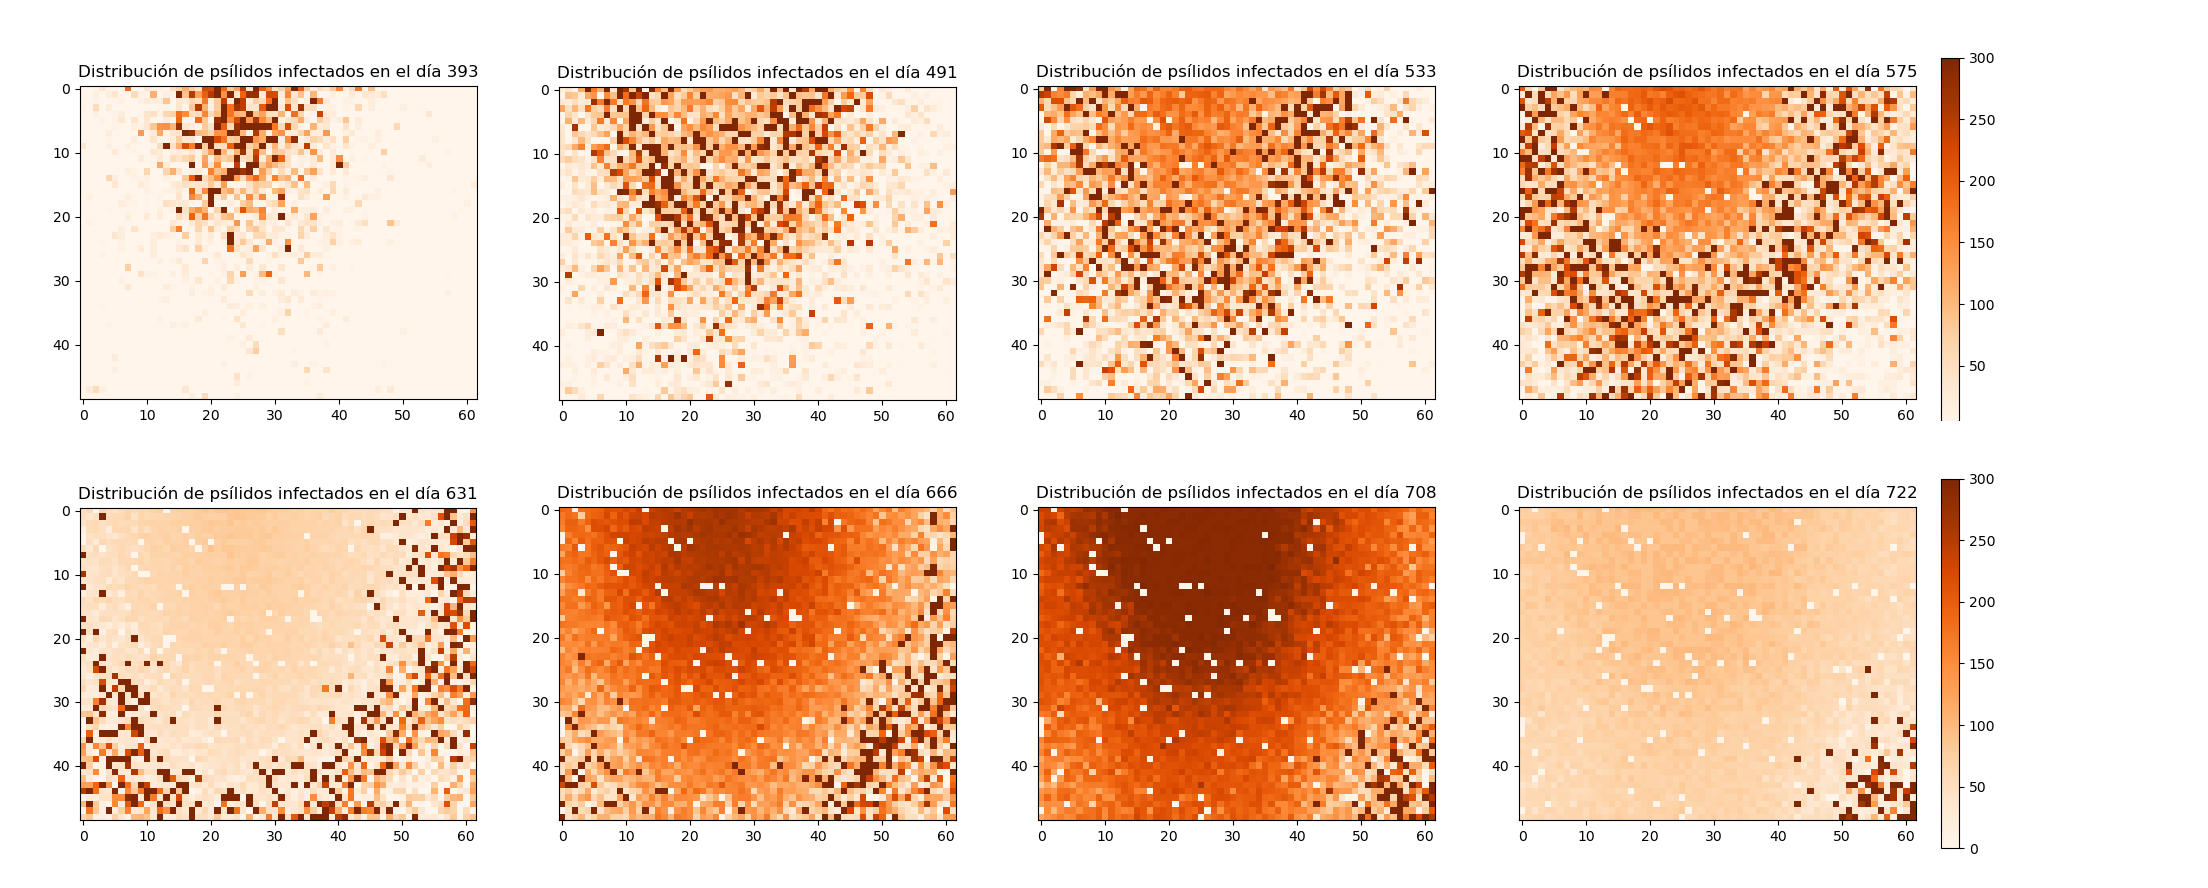
\includegraphics[width=1.05\textwidth,keepaspectratio=true]{images/Imágenes C6/C6-5.png}
\caption{Patrón formado por el crecimiento y distribución de la población de psílidos infecciosos con el pasar de los días.}
\end{figure}


%Códigos todos -------------------------------------------------------------------------------------------------------------------------------------------------------------VIABILIDAD DEL MÉTODO DE MEDICIÓN EN T SOBRE OTROS MÉTODOS
\section{Justificación del \textit{Método en «T»}}

%Hechos:
%ÚNICO:En todas las simulaciones con todas las variables, los psílidos, los asintomáticos, y los sintomáticos son manchas crecientes. Y más aún, los primeros sintomáticos suelen ser el centro de los asintomáticos.
Hasta ahora, no se ha hablado de la relación que tienen las manchas de crecimiento de los distintos tipos de agentes que conforman el sistema. En esta sección se abordará dicha dinámica y se la relacionará con el método de vigilancia propuesto por el protocolo oficial para detectar árboles asintomáticos. Se ha observado en todas las simulaciones que se hicieron, sin importar qué variables se modificaran, ni cómo se modificaran, que los agentes del campo se expanden formando manchas crecientes y concéntricas.
Las primeras apariciones puntuales son las que resultan de la colocación inicial de psílidos, tanto psílidos sanos como infecciosos, estos puntos con psílidos comienzan a convertirse de a poco en una mancha que crece alrededor del lugar donde fueron colocados al principio, este lugar se convierte normalmente en centro de la mancha de psílidos y de todas las que le sucederán. Cuando ha pasado suficiente tiempo, la mancha de psílidos es suficientemente grande y son observadas las primeras apariciones puntuales de árboles asintomáticos en el centro de la mancha de psílidos, y replicando a su antecesora, esta mancha de árboles asintomáticos también comienza a expandirse de a poco, esto mientras la mancha de psílidos totales sigue creciendo. Después de que la mancha de los árboles asintomáticos ha cobrado cierto tamaño, y en el caso de esta simulación, en torno a los 200 días, los primeros brotes puntuales de árboles sintomáticos aparecen, replicando en su crecimiento a las manchas que lo antecedieron. Además, si se hace una distinción entre la mancha de psílidos infecciosos y la de psílidos totales, se puede observar un comportamiento similar.
Lo anterior da como consecuencia que los primeros árboles que presentan síntomas en una huerta suelen ser el centro de la infección, y ese centro es el lugar de arribo de los psílidos y también el lugar a partir del cual los árboles asintomáticos han comenzado a infectarse. A continuación, en la Figura 5.7, se ilustran estas tres fases.
\begin{figure}[H]
\centering
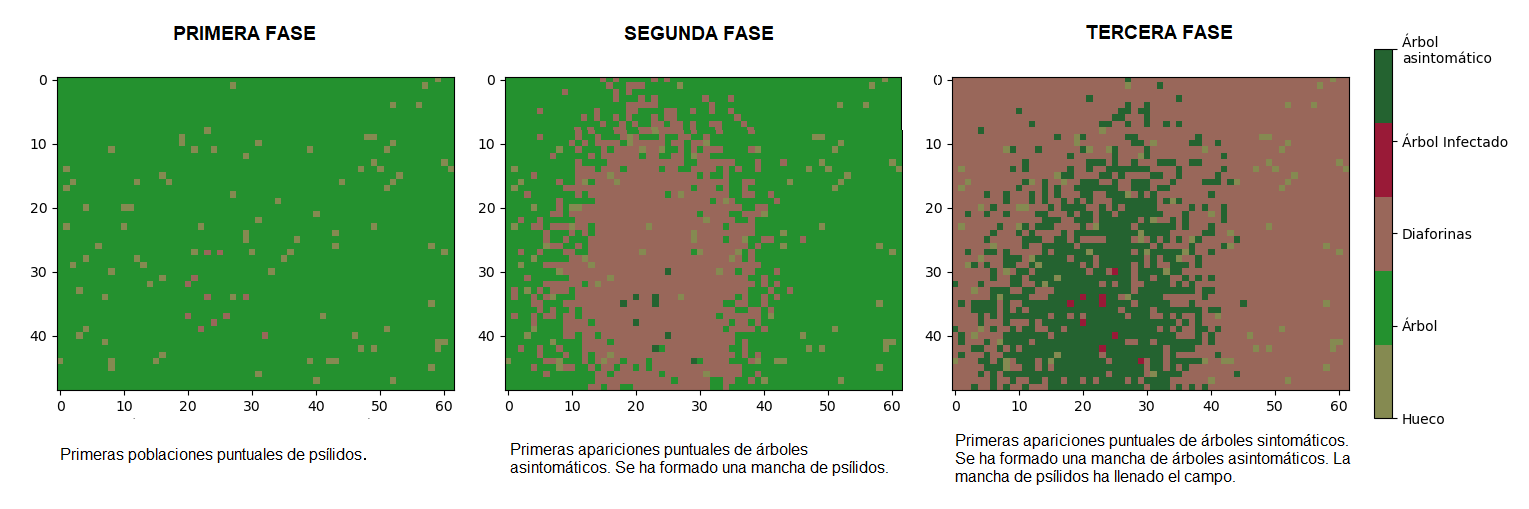
\includegraphics[width=1.05\textwidth,keepaspectratio=true]{images/Imágenes C6/C6-6.png}
\caption{Crecimiento concéntrico de la distribución de psílidos, árboles infectados, y árboles sintomáticos.}
\end{figure}

%Ideas:
Dado que la evidencia consultada indica que los psílidos que llegan a los huertos suelen instalarse en los árboles de los bordes, o cerca de ellos, el método de «revisión en T» del que se habló en el capítulo 3, queda respaldado. Si los psílidos arriban por los bordes y su población crece en manchas, y a estas manchas de psílidos seguirán las manchas de árboles asintomáticos, entonces, los árboles asintomáticos se propagarán también en manchas desde los bordes, y la estrategia de revisión «en T» se ajusta bien a esta característica.
Más aún, se puede establecer que, en general, cuando se detecta un árbol con síntomas, hay una buena probabilidad de que este esté en el centro de la mancha de árboles asintomáticos. Por esta razón sería de interés el calibrar esta simulación en virtud de estar en condiciones de estimar el tamaño de estas manchas asintomáticas en función del tiempo en las huertas reales.
%Propuestas:
Con esta información, se puede asegurar que una buena forma de buscar árboles asintomáticos a partir de la detección de un árbol con síntomas es mediante el método «en T» cuando el árbol esté cerca a los bordes, y en general, si el árbol se encontrase al centro de la huerta, podría extenderse el patrón, de ser una te a ser una cruz como se ve en la figura siguiente (5.8):
\begin{figure}[H]
\centering
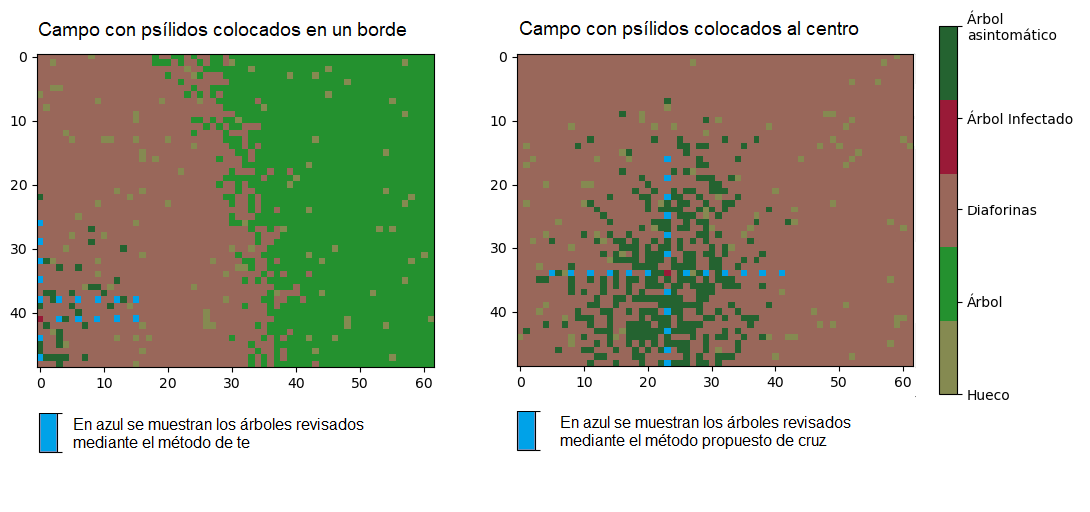
\includegraphics[width=1.05\textwidth,keepaspectratio=true]{images/Imágenes C6/C6-7.png}
\caption{A la izquierda, ilustración del «método en T» descrito en el capítulo tercero. A la derecha, un método propuesto para revisar orígenes de infección al centro.}
\end{figure}
	
%Códigos algunos xd--------------------------------------------------------------------------------------------------------------------------------------------------------LA RELACIÓN ENTRE LOS ASINTOMÁTICOS Y LOS SINTOMÁTICOS
\section{La relación entre árboles asintomáticos y sintomáticos}
%Hechos:
%SEGUNDO: Del mismo modo las gráficas de crecimiento de árboles sintomáticos e infectados son similares salvo un desfase de 200 días, ver árboles Control día 722 -
La primera observación respecto a la relación que existe entre el crecimiento de los árboles asintomáticos y los sintomáticos tiene que ver con el comportamiento descrito anteriormente, en el que la expansión de las manchas de árboles con síntomas sigue a la expansión de los árboles asintomáticos. Este efecto queda de manifiesto cuando se analiza la gráfica del crecimiento de árboles asintomáticos y con síntomas de un huerto sin ningún método de control. El crecimiento de la población de árboles sintomáticos obedece al crecimiento de la población de psílidos, como se ve en la Figura 5.9.
\begin{figure}[H]
\centering
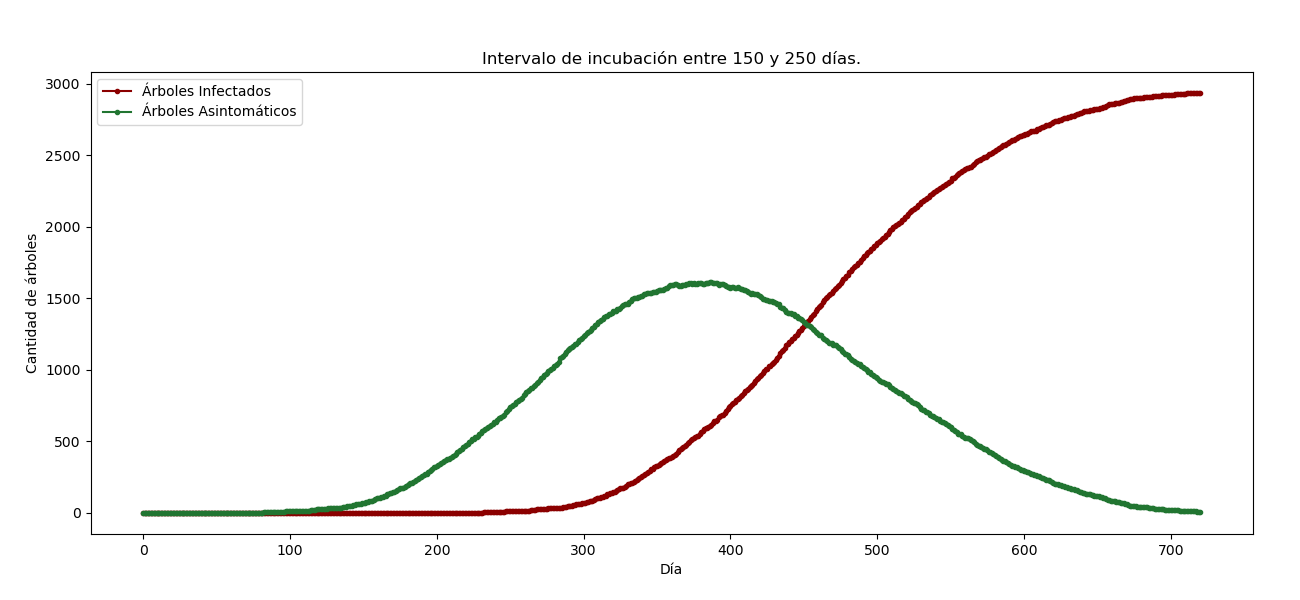
\includegraphics[width=1\textwidth,keepaspectratio=true]{images/Imágenes C6/C6-8.png}
\caption{Gráfica de la cantidad de árboles infectados y sanos, respectivamente, a través del tiempo, para una huerta sin control.}
\end{figure}
%HECHO TERCERO: La gráfica verde es la derivada de la roja desplazada, incluso cuando se aplica el corte
La línea verde está estrechamente relacionada con la trayectoria de la línea roja, esto es que el crecimiento en la población de árboles asintomáticos puede ser asociado con el crecimiento de la población de árboles sintomáticos. El crecimiento de la población del psílido está modelado como una función logística, y la gráfica de los árboles sintomáticos tiene un comportamiento similar al de la gráfica de una función logística. La línea verde de árboles asintomáticos tiene una silueta parecida a la de la distribución logística, la función de densidad de probabilidad cuya función de distribución es justamente la función de distribución logística.

%Idea:
El crecimiento en los árboles sintomáticos puede explicarse mediante el hecho de que, en el modelo, la probabilidad de que un árbol se infecte está solamente dada por la cantidad de psílidos infecciosos que aloje, algo que tiene como consecuencia que la cantidad de psílidos que haya en la huerta, en algún momento, condicionará la cantidad de árboles que se infecten en ese momento, de modo que es por esta razón que el crecimiento de las infecciones en una huerta es una calca del crecimiento de los psílidos infectados en esa misma huerta.
Una línea para continuar la investigación, podría ser la búsqueda de alguna forma analítica de estimar la cantidad de árboles asintomáticos dados los datos de la cantidad de árboles con síntomas.

La relación entre ambas poblaciones de árboles parece estar presente incluso cuando se aplican métodos de control como el pesticida y el corte de árboles sintomáticos. Cuando el pesticida es aplicado, las curvas se aplanan más o menos en función de la intensidad de la aplicación del pesticida, mientras que al hacer uso del corte de árboles sintomáticos, el comportamiento se mantiene a pesar de las reducciones en la población de árboles infectados; a continuación se muestra la gráfica de poblaciones de árboles de una huerta en la que fue aplicado el método de tala.
\begin{figure}[H]
\centering
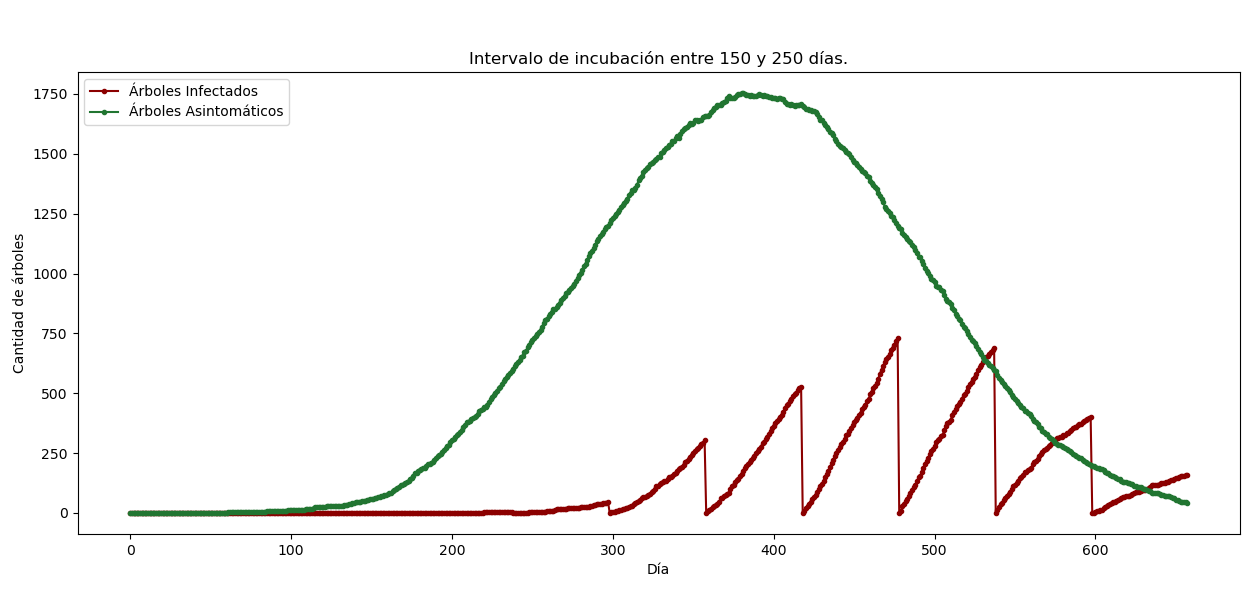
\includegraphics[width=1\textwidth,keepaspectratio=true]{images/Imágenes C6/C6-9.png}
\caption{Gráfica de la cantidad de árboles infectados y sanos, respectivamente, a través del tiempo, para una huerta con eliminación de árboles con síntomas.}
\end{figure}
Este comportamiento implica que de desarrollar una herramienta analítica capaz de estimar la cantidad de árboles asintomáticos en función de la cantidad de árboles sintomáticos, aún en distintos escenarios de control, ésta conservaría tal poder.


%Idea: En lugar de la derivada, graficar asintomáticos vs sintomáticos y dar la curva
\chapter{Conclusiones}

Este capítulo sintetiza los resultados descritos en el anterior. De este trabajo se han desprendido cuatro grandes afirmaciones. En primer lugar, en lo que respecta a los distintos métodos de control, y cómo estos afectan a la dinámica de crecimiento de los árboles asintomáticos, especialmente reduciendo su propagación, se encontró que no existe mejor herramienta de entre las evaluadas, para combatir el crecimiento de la infección, que el uso recurrente de pesticidas. Cuanto mayor mortalidad y frecuencia tengan estos pesticidas, más lento avanza la enfermedad. Este método no precisa el conocer ningún tipo de información sobre la huerta, basta con aplicarlo uniformemente en ella para obtener, de lejos, mucho mejores resultados que en aquellos métodos que sí requieren de estudiar el campo. Finalmente, en consistencia con lo observado en la realidad, este método está lejos de ser infalible, pues sólo sirve para retrasar la propagación, en el mejor de los casos hasta 260 días, pero no sirve para detenerla. Por otro lado, un método que sí se vale de información recabada de la huerta, como lo es el eliminar árboles, tiene un impacto menor, debido a que sólo se aplica a los árboles sintomáticos, cuando la gran mayoría son asintomáticos.

El segundo resultado de interés es el que respecta a la dinámica de los psílidos infecciosos, cuya propagación sigue a la del resto de psílidos salvo por un tiempo de desfase, esto es, que si se estudia en el tiempo la trayectoria del crecimiento de las poblaciones de psílidos, se verá que la trayectoria de los psílidos infecciosos imitará a la del total de psílidos. Además, hay una clara relación entre las regiones con árboles infectados y las regiones con psílidos infecciosos, llegando a ser idénticas las siluetas de estas dos poblaciones. La explicación que se propone es que en las zonas de la huerta con árboles infectados habrá la mayoría de psílidos infecciosos, y que los que lleguen a emigrar a otro árbol, al ser una minoría, no contribuyen en gran medida a formar la mancha de psílidos infecciosos, y luego, cuando algún psílido infeccioso llega a infectar a un árbol, este comenzará a infectar a todos sus habitantes. Es por esta razón que las zonas con psílidos infecciosos y árboles infectados, son casi equivalentes. También se propone que la mancha de psílidos infecciosos está desfasada de la del resto de psílidos porque esta obedece al comportamiento de la mancha de árboles infectados, y a su vez estos árboles infectados no crecen directamente con las dispersión de psílidos sanos, sino que tardan cierto tiempo en infectarse en función de la cantidad de psílidos que alojen y del tiempo que lleven haciéndolo. Esto último explica por qué, en condiciones ideales, la enfermedad se propaga de forma radial, y justifica la siguiente conclusión.
 
Cuando se toman muestras de árboles en alguna región infectada, el método para hacerlo es el «método en t», que se ha descrito detalladamente en el capítulo tercero. Este método comienza tomando muestras a partir de algún árbol que se considere el punto de partida de la infección, y desde él se avanza radialmente hacia los demás árboles en las cuatro direcciones. Este método está justificado porque en las condiciones de esta simulación, la propagación de los psílidos y de las infecciones crece como manchas concéntricas. La última conclusión es la relativa a la relación entre árboles asintomáticos y sintomáticos. Se ha mostrado anteriormente que sin importar los métodos de control y las condiciones de la huerta, el comportamiento del crecimiento de árboles asintomáticos está condicionado siempre por el de los árboles sintomáticos. Esta es una dirección en la que esta investigación puede continuar, buscando una forma rigurosa de calcular la cantidad de árboles asintomáticos a partir de los datos de árboles sintomáticos, de tal forma que sea posible estimar la cantidad de árboles asintomáticos a voluntad.



\appendix % A partir de esta línea van los apéndices. Quitar si no habrá apéndices
\include{formato-a1}

\backmatter  % En esta línea está terminado el trabajo. No quitar
\addcontentsline{toc}{chapter}{Bibliografía} % Agregar Bibliografía al índice
\bibliographystyle{plain}
\bibliography{ref}      % Para utilizar con BibTeX y con un archivo ref.bib

%\begin{thebibliography}{XX} % Por si alguien no quiere utilizar BibTeX
%\end{thebibliography}
\end{document}            % Fin del documento. cualquier texto a partir de esta
                          % línea es ignorado por latex.
